% cd /disks/PROJECT/Mickael/PRESENTATION/JULIA_TP/; pdflatex JULIA_TP.tex; bibtex JULIA_TP; pdflatex JULIA_TP.tex; pdflatex JULIA_TP.tex; gvfs-open JULIA_TP.pdf
% pdflatex JULIA_TP.tex; gvfs-open JULIA_TP.pdf

\documentclass[10pt, xcolors={RGB}, hyperref={pdfpagelabels=false,
        colorlinks=true,
        linkcolor=black,
        urlcolor=black,
        citecolor=black,
        filecolor=black,
        menucolor=black,
        pdftex=true,
        bookmarks=true,
        bookmarksopen=true,
        hyperfootnotes=true}]{beamer}
\pdfpageattr{/Group << /S /Transparency /I true /CS /DeviceRGB>>}
\usepackage[T1]{fontenc}
\usepackage[utf8]{inputenc}
\usepackage{graphicx}
\usepackage{tabularx}
\usepackage{multirow}

\usepackage{pifont}
\usepackage{multicol}

\usepackage{setspace}
\renewcommand{\baselinestretch}{1.25}

\usepackage{helvet}
\renewcommand{\familydefault}{\sfdefault}

\definecolor{dodgerblue}{RGB}{30,144,255}
\definecolor{springgreen3}{RGB}{0,139,69}
\definecolor{springgreen2}{RGB}{0,205,102}
\definecolor{firebrick2}{RGB}{238,44,44}
\definecolor{maroon2}{RGB}{238,48,167}
\definecolor{goldenrod2}{RGB}{238,180,34}
\definecolor{deepskyblue}{RGB}{0,191,255}

\newif\ifblacked\blackedfalse
\ifblacked
    \hypersetup{%
        linkcolor=black,
        urlcolor=black,
        citecolor=black,
        filecolor=black,
        menucolor=black}
    \renewcommand{\thefootnote}{\textcolor{black}{\arabic{footnote}}}
\else
    \hypersetup{%
        linkcolor=dodgerblue,
        urlcolor=firebrick2,
        citecolor=springgreen3,
        filecolor=goldenrod2,
        menucolor=dodgerblue,
        bookmarksopen=true}
    \renewcommand{\thefootnote}{\textcolor{maroon2}{\arabic{footnote}}}
\fi

\usetheme{CambridgeUS}
\useoutertheme{infolines}
\useinnertheme{rectangles}
\setbeamercolor{frametitle}{fg=white, bg=springgreen3!90!black!60!white}
\setbeamercolor{title}{fg=white, bg=springgreen3!50!white}
\setbeamercolor{palette primary}{fg=springgreen3!40!black, bg=springgreen3!50!white}
\setbeamercolor{palette secondary}{fg=springgreen3!30!black, bg=springgreen3!70!white}
\setbeamercolor{palette tertiary}{fg=springgreen3!20!black, bg=springgreen3!90!white}
\setbeamercolor{structure}{fg=springgreen3!70!white}
\setbeamercolor{background canvas}{bg=white}
\setbeamercolor{normal text}{fg=black}
\setbeamercolor{block title}{bg=dodgerblue, fg=white!75!dodgerblue}
\setbeamercolor{example text}{fg=springgreen3}
\setbeamercolor{block title example}{bg=springgreen3, fg=white!75!springgreen3}
\setbeamercolor{alerted text}{fg=firebrick2}
\setbeamercolor{block title alerted}{bg=firebrick2, fg=white!75!firebrick2}

\usepackage{textcomp}
\usepackage{listings}
\usepackage{courier}
\lstset{ %
    backgroundcolor=\color{dodgerblue!2.5!white},       % choose the background color; you must add \usepackage{color} or \usepackage{xcolor}
    basicstyle={\tiny\ttfamily\mdseries},               % the size of the fonts that are used for the code
    breakatwhitespace=true,                             % sets if automatic breaks should only happen at whitespace
    breaklines=true,                                    % sets automatic line breaking
    captionpos=none,                                    % sets the caption-position to bottom
    commentstyle=\color{springgreen3},                  % comment style
    deletekeywords={...},                               % if you want to delete keywords from the given language
    escapeinside={!*}{*!},                              % if you want to add LaTeX within your code
    extendedchars=true,                                 % lets you use non-ASCII characters; for 8-bits encodings only, does not work with UTF-8
    frame=single,                                       % adds a frame around the code
    keepspaces=true,                                    % keeps spaces in text, useful for keeping indentation of code (possibly needs columns=flexible)
    keywordstyle={\color{dodgerblue}\textbf},           % keyword style
    morekeywords={*,...},                               % if you want to add more keywords to the set
    numbers=none,                                       % where to put the line-numbers; possible values are (none, left, right)
    numbersep=10pt,                                     % how far the line-numbers are from the code
    numberstyle=\tiny\color{goldenrod2},                % the style that is used for the line-numbers
    rulecolor=\color{dodgerblue},                       % if not set, the frame-color may be changed on line-breaks within not-black text (e.g. comments (green here))
    showspaces=false,                                   % show spaces everywhere adding particular underscores; it overrides 'showstringspaces'
    showstringspaces=false,                             % underline spaces within strings only
    showtabs=false,                                     % show tabs within strings adding particular underscores
    stepnumber=1,                                       % the step between two line-numbers. If it's 1, each line will be numbered
    stringstyle=\color{maroon2},                        % string literal style
    tabsize=2,                                          % sets default tabsize to 2 spaces
    title=\lstname,                                     % show the filename of files included with \lstinputlisting; also try caption instead of title
    showlines=false,                                    % prints empty lines at the end of listings
    xleftmargin=9mm,                                    % The dimensions are used as extra margins on the left and right
    xrightmargin=9mm,
    upquote=true,
    lineskip=-0.05ex,                                   % Specifies additional space between lines in listings
    aboveskip=2ex,                                      % Define the space above and below displayed listings
    belowskip=4ex,                                      % Define the space above and below displayed listings
    literate=%
        {à}{{\'a}}1
        {é}{{\'e}}1
        {í}{{\'i}}1
        {ó}{{\'o}}1
        {ú}{{\'u}}1
        {Á}{{\'A}}1
        {É}{{\'E}}1
        {Í}{{\'I}}1
        {Ó}{{\'O}}1
        {Ú}{{\'U}}1
        {à}{{\`a}}1
        {è}{{\`e}}1
        {ì}{{\`i}}1
        {ò}{{\`o}}1
        {ù}{{\`u}}1
        {À}{{\`A}}1
        {È}{{\'E}}1
        {Ì}{{\`I}}1
        {Ò}{{\`O}}1
        {Ù}{{\`U}}1
        {ä}{{\"a}}1
        {ë}{{\"e}}1
        {ï}{{\"i}}1
        {ö}{{\"o}}1
        {ü}{{\"u}}1
        {Ä}{{\"A}}1
        {Ë}{{\"E}}1
        {Ï}{{\"I}}1
        {Ö}{{\"O}}1
        {Ü}{{\"U}}1
        {â}{{\^a}}1
        {ê}{{\^e}}1
        {î}{{\^i}}1
        {ô}{{\^o}}1
        {û}{{\^u}}1
        {Â}{{\^A}}1
        {Ê}{{\^E}}1
        {Î}{{\^I}}1
        {Ô}{{\^O}}1
        {Û}{{\^U}}1
        {œ}{{\oe}}1
        {Œ}{{\OE}}1
        {æ}{{\ae}}1
        {Æ}{{\AE}}1
        {ß}{{\ss}}1
        {ç}{{\c c}}1
        {Ç}{{\c C}}1
        {ø}{{\o}}1
        {å}{{\r a}}1
        {Å}{{\r A}}1
}
\lstdefinelanguage{JuliaConsole}{
    morecomment=[l]{\#},
    backgroundcolor=\color{gray!2.5!white},             % choose the background color; you must add \usepackage{color} or \usepackage{xcolor}
    rulecolor=\color{gray!50!white},                    % if not set, the frame-color may be changed on line-breaks within not-black text (e.g. comments (green here))
    alsoletter={>},
    literate=%
    *{\$}{{{\color{black}\bfseries \$}}}1
    {julia>}{{{\color{black}\bfseries julia>}}}6
}
\lstdefinelanguage{Julia}{
    keywordsprefix=\@,
    morekeywords={
        exit, whos, edit, load, is, isa, isequal, typeof, tuple, ntuple, uid, hash, finalizer, convert, promote,
        subtype, typemin, typemax, realmin, realmax, sizeof, eps, promote_type, method_exists, applicable,
        invoke, dlopen, dlsym, system, error, throw, assert, new, Inf, Nan, pi, im, begin, while, for, in, return,
        break, continue, macro, quote, let, if, elseif, else, try, catch, end, bitstype, ccall, do, using, module,
        import, export, importall, baremodule, immutable, local, global, const, Bool, Int, Int8, Int16, Int32,
        Int64, Uint, Uint8, Uint16, Uint32, Uint64, Float32, Float64, Complex64, Complex128, Any, Nothing, None,
        function, type, typealias, abstract, include, require, names, info, warn, workspace
    },
    alsoletter={>},
    sensitive=true,
    morecomment=[l]{\#},
    morecomment=[s]{\#=}{=\#},
    morestring=[b]',
    morestring=[b]",
    literate=%
    *{0}{{{\color{goldenrod2}\textbf{0}}}}1
    {1}{{{\color{goldenrod2}\textbf{1}}}}1
    {2}{{{\color{goldenrod2}\textbf{2}}}}1
    {3}{{{\color{goldenrod2}\textbf{3}}}}1
    {4}{{{\color{goldenrod2}\textbf{4}}}}1
    {5}{{{\color{goldenrod2}\textbf{5}}}}1
    {6}{{{\color{goldenrod2}\textbf{6}}}}1
    {7}{{{\color{goldenrod2}\textbf{7}}}}1
    {8}{{{\color{goldenrod2}\textbf{8}}}}1
    {9}{{{\color{goldenrod2}\textbf{9}}}}1
    {0.0}{{{\color{goldenrod2}\textbf{0.0}}}}3
    {1.0}{{{\color{goldenrod2}\textbf{1.0}}}}3
    {2.0}{{{\color{goldenrod2}\textbf{2.0}}}}3
    {3.0}{{{\color{goldenrod2}\textbf{3.0}}}}3
    {4.0}{{{\color{goldenrod2}\textbf{4.0}}}}3
    {5.0}{{{\color{goldenrod2}\textbf{5.0}}}}3
    {6.0}{{{\color{goldenrod2}\textbf{6.0}}}}3
    {7.0}{{{\color{goldenrod2}\textbf{7.0}}}}3
    {8.0}{{{\color{goldenrod2}\textbf{8.0}}}}3
    {9.0}{{{\color{goldenrod2}\textbf{9.0}}}}3
    {0.1}{{{\color{goldenrod2}\textbf{0.1}}}}3
    {1.1}{{{\color{goldenrod2}\textbf{1.1}}}}3
    {2.1}{{{\color{goldenrod2}\textbf{2.1}}}}3
    {3.1}{{{\color{goldenrod2}\textbf{3.1}}}}3
    {4.1}{{{\color{goldenrod2}\textbf{4.1}}}}3
    {5.1}{{{\color{goldenrod2}\textbf{5.1}}}}3
    {6.1}{{{\color{goldenrod2}\textbf{6.1}}}}3
    {7.1}{{{\color{goldenrod2}\textbf{7.1}}}}3
    {8.1}{{{\color{goldenrod2}\textbf{8.1}}}}3
    {9.1}{{{\color{goldenrod2}\textbf{9.1}}}}3
    {0.2}{{{\color{goldenrod2}\textbf{0.2}}}}3
    {1.2}{{{\color{goldenrod2}\textbf{1.2}}}}3
    {2.2}{{{\color{goldenrod2}\textbf{2.2}}}}3
    {3.2}{{{\color{goldenrod2}\textbf{3.2}}}}3
    {4.2}{{{\color{goldenrod2}\textbf{4.2}}}}3
    {5.2}{{{\color{goldenrod2}\textbf{5.2}}}}3
    {6.2}{{{\color{goldenrod2}\textbf{6.2}}}}3
    {7.2}{{{\color{goldenrod2}\textbf{7.2}}}}3
    {8.2}{{{\color{goldenrod2}\textbf{8.2}}}}3
    {9.2}{{{\color{goldenrod2}\textbf{9.2}}}}3
    {0.3}{{{\color{goldenrod2}\textbf{0.3}}}}3
    {1.3}{{{\color{goldenrod2}\textbf{1.3}}}}3
    {2.3}{{{\color{goldenrod2}\textbf{2.3}}}}3
    {3.3}{{{\color{goldenrod2}\textbf{3.3}}}}3
    {4.3}{{{\color{goldenrod2}\textbf{4.3}}}}3
    {5.3}{{{\color{goldenrod2}\textbf{5.3}}}}3
    {6.3}{{{\color{goldenrod2}\textbf{6.3}}}}3
    {7.3}{{{\color{goldenrod2}\textbf{7.3}}}}3
    {8.3}{{{\color{goldenrod2}\textbf{8.3}}}}3
    {9.3}{{{\color{goldenrod2}\textbf{9.3}}}}3
    {0.4}{{{\color{goldenrod2}\textbf{0.4}}}}3
    {1.4}{{{\color{goldenrod2}\textbf{1.4}}}}3
    {2.4}{{{\color{goldenrod2}\textbf{2.4}}}}3
    {3.4}{{{\color{goldenrod2}\textbf{3.4}}}}3
    {4.4}{{{\color{goldenrod2}\textbf{4.4}}}}3
    {5.4}{{{\color{goldenrod2}\textbf{5.4}}}}3
    {6.4}{{{\color{goldenrod2}\textbf{6.4}}}}3
    {7.4}{{{\color{goldenrod2}\textbf{7.4}}}}3
    {8.4}{{{\color{goldenrod2}\textbf{8.4}}}}3
    {9.4}{{{\color{goldenrod2}\textbf{9.4}}}}3
    {0.5}{{{\color{goldenrod2}\textbf{0.5}}}}3
    {1.5}{{{\color{goldenrod2}\textbf{1.5}}}}3
    {2.5}{{{\color{goldenrod2}\textbf{2.5}}}}3
    {3.5}{{{\color{goldenrod2}\textbf{3.5}}}}3
    {4.5}{{{\color{goldenrod2}\textbf{4.5}}}}3
    {5.5}{{{\color{goldenrod2}\textbf{5.5}}}}3
    {6.5}{{{\color{goldenrod2}\textbf{6.5}}}}3
    {7.5}{{{\color{goldenrod2}\textbf{7.5}}}}3
    {8.5}{{{\color{goldenrod2}\textbf{8.5}}}}3
    {9.5}{{{\color{goldenrod2}\textbf{9.5}}}}3
    {0.6}{{{\color{goldenrod2}\textbf{0.6}}}}3
    {1.6}{{{\color{goldenrod2}\textbf{1.6}}}}3
    {2.6}{{{\color{goldenrod2}\textbf{2.6}}}}3
    {3.6}{{{\color{goldenrod2}\textbf{3.6}}}}3
    {4.6}{{{\color{goldenrod2}\textbf{4.6}}}}3
    {5.6}{{{\color{goldenrod2}\textbf{5.6}}}}3
    {6.6}{{{\color{goldenrod2}\textbf{6.6}}}}3
    {7.6}{{{\color{goldenrod2}\textbf{7.6}}}}3
    {8.6}{{{\color{goldenrod2}\textbf{8.6}}}}3
    {9.6}{{{\color{goldenrod2}\textbf{9.6}}}}3
    {0.7}{{{\color{goldenrod2}\textbf{0.7}}}}3
    {1.7}{{{\color{goldenrod2}\textbf{1.7}}}}3
    {2.7}{{{\color{goldenrod2}\textbf{2.7}}}}3
    {3.7}{{{\color{goldenrod2}\textbf{3.7}}}}3
    {4.7}{{{\color{goldenrod2}\textbf{4.7}}}}3
    {5.7}{{{\color{goldenrod2}\textbf{5.7}}}}3
    {6.7}{{{\color{goldenrod2}\textbf{6.7}}}}3
    {7.7}{{{\color{goldenrod2}\textbf{7.7}}}}3
    {8.7}{{{\color{goldenrod2}\textbf{8.7}}}}3
    {9.7}{{{\color{goldenrod2}\textbf{9.7}}}}3
    {0.8}{{{\color{goldenrod2}\textbf{0.8}}}}3
    {1.8}{{{\color{goldenrod2}\textbf{1.8}}}}3
    {2.8}{{{\color{goldenrod2}\textbf{2.8}}}}3
    {3.8}{{{\color{goldenrod2}\textbf{3.8}}}}3
    {4.8}{{{\color{goldenrod2}\textbf{4.8}}}}3
    {5.8}{{{\color{goldenrod2}\textbf{5.8}}}}3
    {6.8}{{{\color{goldenrod2}\textbf{6.8}}}}3
    {7.8}{{{\color{goldenrod2}\textbf{7.8}}}}3
    {8.8}{{{\color{goldenrod2}\textbf{8.8}}}}3
    {9.8}{{{\color{goldenrod2}\textbf{9.8}}}}3
    {0.9}{{{\color{goldenrod2}\textbf{0.9}}}}3
    {1.9}{{{\color{goldenrod2}\textbf{1.9}}}}3
    {2.9}{{{\color{goldenrod2}\textbf{2.9}}}}3
    {3.9}{{{\color{goldenrod2}\textbf{3.9}}}}3
    {4.9}{{{\color{goldenrod2}\textbf{4.9}}}}3
    {5.9}{{{\color{goldenrod2}\textbf{5.9}}}}3
    {6.9}{{{\color{goldenrod2}\textbf{6.9}}}}3
    {7.9}{{{\color{goldenrod2}\textbf{7.9}}}}3
    {8.9}{{{\color{goldenrod2}\textbf{8.9}}}}3
    {9.9}{{{\color{goldenrod2}\textbf{9.9}}}}3
    {Inf}{{{\color{goldenrod2}\textbf{Inf}}}}3
    {Int32}{{{\color{springgreen3}\textbf{Int32}}}}5
    {Int64}{{{\color{springgreen3}\textbf{Int64}}}}5
    {Float32}{{{\color{springgreen3}\textbf{Float32}}}}7
    {Float64}{{{\color{springgreen3}\textbf{Float64}}}}7
    {ASCIIString}{{{\color{springgreen3}\textbf{ASCIIString}}}}{11}
    {Char}{{{\color{springgreen3}\textbf{Char}}}}4
    {Bool}{{{\color{springgreen3}\textbf{Bool}}}}4
    {Any}{{{\color{springgreen3}\textbf{Any}}}}3
    {+}{{{\color{deepskyblue!85!black}\textbf{+}}}}1
    {-}{{{\color{deepskyblue!85!black}\textbf{-}}}}1
    {*}{{{\color{deepskyblue!85!black}\textbf{*}}}}1
    {/}{{{\color{deepskyblue!85!black}\textbf{/}}}}1
    {\%>\%}{{{\color{deepskyblue!85!black}\textbf{\%>\%}}}}3
    {(}{{{\color{deepskyblue!85!black}\textbf{(}}}}1
    {)}{{{\color{deepskyblue!85!black}\textbf{)}}}}1
    {[}{{{\color{deepskyblue!85!black}\textbf{[}}}}1
    {]}{{{\color{deepskyblue!85!black}\textbf{]}}}}1
    {\{}{{{\color{deepskyblue!85!black}\textbf{\{}}}}1
    {\}}{{{\color{deepskyblue!85!black}\textbf{\}}}}}1
    {julia>}{{{\color{black}\bfseries julia>}}}6
    {shell>}{{{\color{firebrick2}\bfseries shell>}}}6
    {help?>}{{{\color{goldenrod2}\bfseries help?>}}}6
    {Pkg.status}{{{\color{dodgerblue}\textbf{Pkg.status}}}}{10}
    {Pkg.installed}{{{\color{dodgerblue}\textbf{Pkg.installed}}}}{13}
    {Pkg.update}{{{\color{dodgerblue}\textbf{Pkg.update}}}}{10}
    {Pkg.add}{{{\color{dodgerblue}\textbf{Pkg.add}}}}7
    {Pkg.clone}{{{\color{dodgerblue}\textbf{Pkg.clone}}}}9
    {Pkg.rm}{{{\color{dodgerblue}\textbf{Pkg.rm}}}}6
}
\lstdefinelanguage{R}{
    % backgroundcolor=\color{dodgerblue!2.5!white},       % choose the background color; you must add \usepackage{color} or \usepackage{xcolor}
    % rulecolor=\color{dodgerblue!50!white},              % if not set, the frame-color may be changed on line-breaks within not-black text (e.g. comments (green here))
    % commentstyle=\color{springgreen3},                  % comment style
    % keywordstyle={\color{dodgerblue}\textbf},           % keyword style
    % numberstyle=\scriptsize\color{goldenrod2},          % the style that is used for the line-numbers
    % stringstyle=\color{maroon2},                        % string literal style
    morekeywords={
        if, else, repeat, while, function, for, in, next, break, TRUE, FALSE, NULL, NA, NaN, abbreviate, abline, abs, acf, acos, acosh, addmargins, aggregate, agrep,
        alarm, alias, alist, all, anova, any, aov, aperm, append, apply, approx, approxfun, apropos, ar, args, arima, array, arrows, asin, asinh, assign, assocplot, atan,
        atanh, attach, attr, attributes, autoload, autoloader, ave, axis, backsolve, barplot, basename, beta, bindtextdomain, binomial, biplot, bitmap, bmp, body, box,
        boxplot, bquote, break, browser, builtins, bxp, by, bzfile, c call, cancor, capabilities, casefold, cat, category, cbind, ccf, ceiling, character, charmatch,
        chartr, chol, choose, chull, citation, class, close, cm, cmdscale, codes, coef, coefficients, col, colnames, colors, colorspaces, colours, comment, complex,
        confint, conflicts, contour, contrasts, contributors, convolve, cophenetic, coplot, cor, cos, cosh, cov, covratio, cpgram, crossprod, cummax, cummin, cumprod,
        cumsum, curve, cut, cutree, cycle, data, dataentry, date, dbeta, dbinom, dcauchy, dchisq, de, debug, debugger, decompose, delay, deltat, demo, dendrapply,
        density, deparse, deriv, det, detach, determinant, deviance, dexp, df, dfbeta, dfbetas, dffits, dgamma, dgeom, dget, dhyper, diag, diff, diffinv, difftime,
        digamma, dim, dimnames, dir, dirname, dist, dlnorm, dlogis, dmultinom, dnbinom, dnorm, dotchart, double, dpois, dput, drop, dsignrank, dt, dump, dunif, duplicated,
        dweibull, dwilcox, eapply, ecdf, edit, effects, eigen, emacs, embed, end, environment, eval, evalq, example, exists, exp, expression, factanal, factor, factorial,
        family, fft, fifo, file, filter, find, fitted, fivenum, fix, floor, flush, for, force, formals, format, formula, forwardsolve, fourfoldplot, frame, frequency,
        ftable, function, gamma, gaussian, gc, gcinfo, gctorture, get, getenv, geterrmessage, gettext, gettextf, getwd, gl, glm, globalenv, gray, grep, grey, grid, gsub,
        gzcon, gzfile, hat, hatvalues, hcl, hclust, head, heatmap, help, hist, history, hsv, httpclient, iconv, iconvlist, identical, identify, if, ifelse, image,
        influence, inherits, integer, integrate, interaction, interactive, intersect, invisible, isoreg, jitter, jpeg, julian, kappa, kernapply, kernel, kmeans, knots,
        kronecker, ksmooth, labels, lag, lapply, layout, lbeta, lchoose, lcm, legend, length, letters, levels, lfactorial, lgamma, library, licence, license, line, lines,
        list, lm, load, loadhistory, loadings, local, locator, loess, log, logb, logical, loglin, lowess, ls, lsfit, machine, mad, mahalanobis, makepredictcall, manova,
        mapply, match, matlines, matplot, matpoints, matrix, max, mean, median, medpolish, menu, merge, message, methods, mget, min, missing, mode, monthplot, months,
        mosaicplot, mtext, mvfft, names, napredict, naprint, naresid, nargs, nchar, ncol, next, nextn, ngettext, nlevels, nlm, nls, noquote, nrow, numeric, objects, offset,
        open, optim, optimise, optimize, options, order, ordered, outer, pacf, page, pairlist, pairs, palette, par, parse, paste, pbeta, pbinom, pbirthday, pcauchy, pchisq,
        pdf, pentagamma, person, persp, pexp, pf, pgamma, pgeom, phyper, pi, pico, pictex, pie, piechart, pipe, plclust, plnorm, plogis, plot, pmatch, pmax, pmin, pnbinom,
        png, pnorm, points, poisson, poly, polygon, polym, polyroot, postscript, power, ppoints, ppois, ppr, prcomp, predict, preplot, pretty, princomp, print, prmatrix,
        prod, profile, profiler, proj, promax, prompt, provide, psigamma, psignrank, pt, ptukey, punif, pweibull, pwilcox, q qbeta, qbinom, qbirthday, qcauchy, qchisq, qexp,
        qf, qgamma, qgeom, qhyper, qlnorm, qlogis, qnbinom, qnorm, qpois, qqline, qqnorm, qqplot, qr, qsignrank, qt, qtukey, quantile, quarters, quasi, quasibinomial,
        quasipoisson, quit, qunif, quote, qweibull, qwilcox, rainbow, range, rank, raw, rbeta, rbind, rbinom, rcauchy, rchisq, readline, real, recover, rect, reformulate,
        regexpr, relevel, remove, reorder, rep, repeat, replace, replicate, replications, require, reshape, resid, residuals, restart, return, rev, rexp, rf, rgamma, rgb,
        rgeom, rhyper, rle, rlnorm, rlogis, rm, rmultinom, rnbinom, rnorm, round, row, rownames, rowsum, rpois, rsignrank, rstandard, rstudent, rt, rug, runif, runmed,
        rweibull, rwilcox, sample, sapply, save, savehistory, scale, scan, screen, screeplot, sd, search, searchpaths, seek, segments, seq, sequence, serialize, setdiff,
        setequal, setwd, shell, sign, signif, sin, single, sinh, sink, smooth, solve, sort, source, spectrum, spline, splinefun, split, sprintf, sqrt, stack, stars, start,
        stderr, stdin, stdout, stem, step, stepfun, stl, stop, stopifnot, str, strftime, strheight, stripchart, strptime, strsplit, strtrim, structure, strwidth, strwrap,
        sub, subset, substitute, substr, substring, sum, summary, sunflowerplot, supsmu, svd, sweep, switch, symbols, symnum, system, t table, tabulate, tail, tan, tanh,
        tapply, tempdir, tempfile, termplot, terms, tetragamma, text, time, title, toeplitz, tolower, topenv, toupper, trace, traceback, transform, trigamma, trunc,
        truncate, try, ts, tsdiag, tsp, typeof, unclass, undebug, union, unique, uniroot, unix, unlink, unlist, unname, unserialize, unsplit, unstack, untrace, unz,
        update, upgrade, url, var, varimax, vcov, vector, version, vi, vignette, warning, warnings, weekdays, weights, which, while, window, windows, with, write,
        wsbrowser, xedit, xemacs, xfig, xinch, xor, xtabs, xyinch, yinch, zapsmall,
        ggplot, ggvis
    },
    sensitive=true,
    morecomment=[l]{\#},
    morestring=[b]',
    morestring=[b]",
    literate=%
    *{0}{{{\color{goldenrod2}\textbf{0}}}}1
    {1}{{{\color{goldenrod2}\textbf{1}}}}1
    {2}{{{\color{goldenrod2}\textbf{2}}}}1
    {3}{{{\color{goldenrod2}\textbf{3}}}}1
    {4}{{{\color{goldenrod2}\textbf{4}}}}1
    {5}{{{\color{goldenrod2}\textbf{5}}}}1
    {6}{{{\color{goldenrod2}\textbf{6}}}}1
    {7}{{{\color{goldenrod2}\textbf{7}}}}1
    {8}{{{\color{goldenrod2}\textbf{8}}}}1
    {9}{{{\color{goldenrod2}\textbf{9}}}}1
    {0.0}{{{\color{goldenrod2}\textbf{0.0}}}}3
    {1.0}{{{\color{goldenrod2}\textbf{1.0}}}}3
    {2.0}{{{\color{goldenrod2}\textbf{2.0}}}}3
    {3.0}{{{\color{goldenrod2}\textbf{3.0}}}}3
    {4.0}{{{\color{goldenrod2}\textbf{4.0}}}}3
    {5.0}{{{\color{goldenrod2}\textbf{5.0}}}}3
    {6.0}{{{\color{goldenrod2}\textbf{6.0}}}}3
    {7.0}{{{\color{goldenrod2}\textbf{7.0}}}}3
    {8.0}{{{\color{goldenrod2}\textbf{8.0}}}}3
    {9.0}{{{\color{goldenrod2}\textbf{9.0}}}}3
    {0.1}{{{\color{goldenrod2}\textbf{0.1}}}}3
    {1.1}{{{\color{goldenrod2}\textbf{1.1}}}}3
    {2.1}{{{\color{goldenrod2}\textbf{2.1}}}}3
    {3.1}{{{\color{goldenrod2}\textbf{3.1}}}}3
    {4.1}{{{\color{goldenrod2}\textbf{4.1}}}}3
    {5.1}{{{\color{goldenrod2}\textbf{5.1}}}}3
    {6.1}{{{\color{goldenrod2}\textbf{6.1}}}}3
    {7.1}{{{\color{goldenrod2}\textbf{7.1}}}}3
    {8.1}{{{\color{goldenrod2}\textbf{8.1}}}}3
    {9.1}{{{\color{goldenrod2}\textbf{9.1}}}}3
    {0.2}{{{\color{goldenrod2}\textbf{0.2}}}}3
    {1.2}{{{\color{goldenrod2}\textbf{1.2}}}}3
    {2.2}{{{\color{goldenrod2}\textbf{2.2}}}}3
    {3.2}{{{\color{goldenrod2}\textbf{3.2}}}}3
    {4.2}{{{\color{goldenrod2}\textbf{4.2}}}}3
    {5.2}{{{\color{goldenrod2}\textbf{5.2}}}}3
    {6.2}{{{\color{goldenrod2}\textbf{6.2}}}}3
    {7.2}{{{\color{goldenrod2}\textbf{7.2}}}}3
    {8.2}{{{\color{goldenrod2}\textbf{8.2}}}}3
    {9.2}{{{\color{goldenrod2}\textbf{9.2}}}}3
    {0.3}{{{\color{goldenrod2}\textbf{0.3}}}}3
    {1.3}{{{\color{goldenrod2}\textbf{1.3}}}}3
    {2.3}{{{\color{goldenrod2}\textbf{2.3}}}}3
    {3.3}{{{\color{goldenrod2}\textbf{3.3}}}}3
    {4.3}{{{\color{goldenrod2}\textbf{4.3}}}}3
    {5.3}{{{\color{goldenrod2}\textbf{5.3}}}}3
    {6.3}{{{\color{goldenrod2}\textbf{6.3}}}}3
    {7.3}{{{\color{goldenrod2}\textbf{7.3}}}}3
    {8.3}{{{\color{goldenrod2}\textbf{8.3}}}}3
    {9.3}{{{\color{goldenrod2}\textbf{9.3}}}}3
    {0.4}{{{\color{goldenrod2}\textbf{0.4}}}}3
    {1.4}{{{\color{goldenrod2}\textbf{1.4}}}}3
    {2.4}{{{\color{goldenrod2}\textbf{2.4}}}}3
    {3.4}{{{\color{goldenrod2}\textbf{3.4}}}}3
    {4.4}{{{\color{goldenrod2}\textbf{4.4}}}}3
    {5.4}{{{\color{goldenrod2}\textbf{5.4}}}}3
    {6.4}{{{\color{goldenrod2}\textbf{6.4}}}}3
    {7.4}{{{\color{goldenrod2}\textbf{7.4}}}}3
    {8.4}{{{\color{goldenrod2}\textbf{8.4}}}}3
    {9.4}{{{\color{goldenrod2}\textbf{9.4}}}}3
    {0.5}{{{\color{goldenrod2}\textbf{0.5}}}}3
    {1.5}{{{\color{goldenrod2}\textbf{1.5}}}}3
    {2.5}{{{\color{goldenrod2}\textbf{2.5}}}}3
    {3.5}{{{\color{goldenrod2}\textbf{3.5}}}}3
    {4.5}{{{\color{goldenrod2}\textbf{4.5}}}}3
    {5.5}{{{\color{goldenrod2}\textbf{5.5}}}}3
    {6.5}{{{\color{goldenrod2}\textbf{6.5}}}}3
    {7.5}{{{\color{goldenrod2}\textbf{7.5}}}}3
    {8.5}{{{\color{goldenrod2}\textbf{8.5}}}}3
    {9.5}{{{\color{goldenrod2}\textbf{9.5}}}}3
    {0.6}{{{\color{goldenrod2}\textbf{0.6}}}}3
    {1.6}{{{\color{goldenrod2}\textbf{1.6}}}}3
    {2.6}{{{\color{goldenrod2}\textbf{2.6}}}}3
    {3.6}{{{\color{goldenrod2}\textbf{3.6}}}}3
    {4.6}{{{\color{goldenrod2}\textbf{4.6}}}}3
    {5.6}{{{\color{goldenrod2}\textbf{5.6}}}}3
    {6.6}{{{\color{goldenrod2}\textbf{6.6}}}}3
    {7.6}{{{\color{goldenrod2}\textbf{7.6}}}}3
    {8.6}{{{\color{goldenrod2}\textbf{8.6}}}}3
    {9.6}{{{\color{goldenrod2}\textbf{9.6}}}}3
    {0.7}{{{\color{goldenrod2}\textbf{0.7}}}}3
    {1.7}{{{\color{goldenrod2}\textbf{1.7}}}}3
    {2.7}{{{\color{goldenrod2}\textbf{2.7}}}}3
    {3.7}{{{\color{goldenrod2}\textbf{3.7}}}}3
    {4.7}{{{\color{goldenrod2}\textbf{4.7}}}}3
    {5.7}{{{\color{goldenrod2}\textbf{5.7}}}}3
    {6.7}{{{\color{goldenrod2}\textbf{6.7}}}}3
    {7.7}{{{\color{goldenrod2}\textbf{7.7}}}}3
    {8.7}{{{\color{goldenrod2}\textbf{8.7}}}}3
    {9.7}{{{\color{goldenrod2}\textbf{9.7}}}}3
    {0.8}{{{\color{goldenrod2}\textbf{0.8}}}}3
    {1.8}{{{\color{goldenrod2}\textbf{1.8}}}}3
    {2.8}{{{\color{goldenrod2}\textbf{2.8}}}}3
    {3.8}{{{\color{goldenrod2}\textbf{3.8}}}}3
    {4.8}{{{\color{goldenrod2}\textbf{4.8}}}}3
    {5.8}{{{\color{goldenrod2}\textbf{5.8}}}}3
    {6.8}{{{\color{goldenrod2}\textbf{6.8}}}}3
    {7.8}{{{\color{goldenrod2}\textbf{7.8}}}}3
    {8.8}{{{\color{goldenrod2}\textbf{8.8}}}}3
    {9.8}{{{\color{goldenrod2}\textbf{9.8}}}}3
    {0.9}{{{\color{goldenrod2}\textbf{0.9}}}}3
    {1.9}{{{\color{goldenrod2}\textbf{1.9}}}}3
    {2.9}{{{\color{goldenrod2}\textbf{2.9}}}}3
    {3.9}{{{\color{goldenrod2}\textbf{3.9}}}}3
    {4.9}{{{\color{goldenrod2}\textbf{4.9}}}}3
    {5.9}{{{\color{goldenrod2}\textbf{5.9}}}}3
    {6.9}{{{\color{goldenrod2}\textbf{6.9}}}}3
    {7.9}{{{\color{goldenrod2}\textbf{7.9}}}}3
    {8.9}{{{\color{goldenrod2}\textbf{8.9}}}}3
    {9.9}{{{\color{goldenrod2}\textbf{9.9}}}}3
    {Inf}{{{\color{goldenrod2}\textbf{Inf}}}}3
    {+}{{{\color{deepskyblue!85!black}\textbf{+}}}}1
    {-}{{{\color{deepskyblue!85!black}\textbf{-}}}}1
    {*}{{{\color{deepskyblue!85!black}\textbf{*}}}}1
    {/}{{{\color{deepskyblue!85!black}\textbf{/}}}}1
    {\%>\%}{{{\color{deepskyblue!85!black}\textbf{\%>\%}}}}3
    {R>}{{{\color{black}\bfseries R>}}}2
    {<-}{{{\color{black}\bfseries <-}}}2
    {(}{{{\color{deepskyblue!85!black}\textbf{(}}}}1
    {)}{{{\color{deepskyblue!85!black}\textbf{)}}}}1
    {[}{{{\color{deepskyblue!85!black}\textbf{[}}}}1
    {]}{{{\color{deepskyblue!85!black}\textbf{]}}}}1
    {\{}{{{\color{deepskyblue!85!black}\textbf{\{}}}}1
    {\}}{{{\color{deepskyblue!85!black}\textbf{\}}}}}1
}
\usepackage{etoolbox}
\makeatletter
\patchcmd{\lsthk@SelectCharTable}{%
  \lst@ifbreaklines\lst@Def{`)}{\lst@breakProcessOther)}\fi
}{%
}{
}{
}
\makeatother

\setlength{\headheight}{15pt}
\setlength{\abovecaptionskip}{0pt}
\setlength{\tabcolsep}{10pt} % default

\newlength{\wideitemsep}
\setlength{\wideitemsep}{.5\itemsep}
\addtolength{\wideitemsep}{-7pt}
\let\olditem\item
\newcommand{\items}{\setlength{\itemsep}{\wideitemsep}\olditem}

\newcommand\bref[2]{\hyperref[#1]{#2~\ref*{#1}}}
\newcommand\cmd[1]{\texttt{\color{black}\textbf{#1}}}
\newcommand\cmdb[1]{\texttt{\color{dodgerblue}\textbf{#1}}}
\newcommand\cmdr[1]{\texttt{\color{firebrick2}\textbf{#1}}}
\newcommand\cmdg[1]{\texttt{\color{springgreen3}\textbf{#1}}}
\newcommand\cmdy[1]{\texttt{\color{goldenrod2}\textbf{#1}}}

\newcommand\pql{{\rmfamily \textbf{\color{goldenrod2}``}}}
\newcommand\pqr{{\rmfamily \textbf{\color{goldenrod2}''}}}

\newcommand\pq[3]{{\rmfamily \textbf{\color{#3}``}}#1{\rmfamily \textbf{\color{#3}''}} - \textcolor{#3}{#2}}

\newenvironment{bquote}[1]
    {\begin{quotation}
    \vspace{10pt}
    \newcommand{\bqauthor}{\normalfont \begin{quote}\begin{flushright}--- #1\end{flushright}\end{quote}}
    \rmfamily \itshape {\huge\textbf{``}}
    }
    {{\huge\textbf{''}}
    \bqauthor
    \end{quotation}
    }

\usepackage[english, francais]{babel}
\selectlanguage{francais}

\AtBeginSection[]
{
  \begin{frame}
    \frametitle{Sommaire}
    \tableofcontents[sectionstyle=show/hide, subsectionstyle=show/hide/hide, subsubsectionstyle=hide/hide/hide]
  \end{frame}
}
% \AtBeginSubsection[]
% {
    % \begin{frame}
        % \frametitle{Sommaire}
        % \tableofcontents[sectionstyle=show/shaded, subsectionstyle=show/shaded/hide, subsubsectionstyle=show/shaded/hide]
    % \end{frame}
% }

\newcommand{\R}{\protect
\includegraphics[height=0.5cm, keepaspectratio]{./Logos/Rlogo.png}}
\newcommand{\Julia}{\protect{\raisebox{-0.5ex}{
\includegraphics[height=0.5cm, keepaspectratio]{./Logos/logo_julia.pdf}}}}

\setbeamertemplate{navigation symbols}{}


\date{\today}
\author[Mickaël Canouil]{\texorpdfstring{Mickaël Canouil\\ \vskip -0.25cm \href{mailto:mickael.canouil@cnrs.fr}{{\scriptsize mickael.canouil@cnrs.fr}}}{Mickaël Canouil}}
\institute[CNRS UMR 8199]{\textcolor{dodgerblue}{\textbf{G}}énomique \textcolor{dodgerblue}{\textbf{I}}ntégrative et \textcolor{dodgerblue}{\textbf{M}}odélisation des \textcolor{dodgerblue}{\textbf{M}}aladies \textcolor{dodgerblue}{\textbf{M}}étaboliques (CNRS UMR 8199)\linebreak
            Institut de Biologie de Lille}
% \institute[UMR 8199]{Integrative Genomics and Modelization of Metabolic Diseases (CNRS UMR 8199)\linebreak
            % Institut de Biologie de Lille}
\titlegraphic{
\includegraphics[height=1cm, keepaspectratio]{./Logos/logo_cnrs.pdf}\hspace{2cm}
\includegraphics[height=1cm, keepaspectratio]{./Logos/logo_egid.pdf}}

\title[\texorpdfstring{\raisebox{-0.5ex}{
\includegraphics[height=0.25cm, keepaspectratio]{./Logos/logo_julia.pdf}}}{}]{\texorpdfstring{Initiation\\\vspace{-1.5ex}{\smallà}\\ \raisebox{-0.5ex}{
\includegraphics[height=2cm, keepaspectratio]{./Logos/logo_julia.pdf}}}{}}


\graphicspath{{/disks/PROJECT/Mickael/PRESENTATION/JULIA_PremiersPas/figures/}}





\begin{document}
\maketitle
\begin{frame}{Sommaire}
    \begin{multicols}{2}
        \tableofcontents[sectionstyle=show/show, subsectionstyle=hide/hide/hide, subsubsectionstyle=hide/hide/hide, sections={1-5}]
        \columnbreak
        \tableofcontents[sectionstyle=show/show, subsectionstyle=hide/hide/hide, subsubsectionstyle=hide/hide/hide, sections={6-10}]
    \end{multicols}
\end{frame}


\section{Introduction}
\subsection{Présentation}
\begin{frame}{Présentation}
    \par{{\Julia} est un langage (2013) sous licence libre et open source \href{https://github.com/JuliaLang/julia/blob/master/LICENSE.md}{MIT}, destiné au calcul scientifique.}
    \begin{itemize}
        \item Langage compilé à la volée (JIT compiler).
        \item Calcul parallèle et distribué.
        \item Performance proche des langages compilés comme le C.
        \item Support des caractères Unicode, incluant l'UTF-8.
        \item Appel de fonctions C et Fortran sans API extérieure (C++ via paquet).
        \item Appel de fonctions Python via le paquet \href{https://github.com/stevengj/PyCall.jl}{PyCall}.
        \item Macros et Metaprogrammation.
    \end{itemize}
\end{frame}

\subsection{Julia et R}
\begin{frame}{Julia et R: Similarités}
    \begin{itemize}
        \item "Julia is a \textbf{high-level}, high-performance \textbf{dynamic programming} language for technical computing."
            \begin{description}
                \item[High-level] Fonctionne sur des éléments atomiques, des vecteurs, matrices, listes, etc.
                \item[Dynamic programming] Présence de type/classe. Les fonctions peuvent être définies de façon interactive.
            \end{description}
        \item "\textbf{defining functions and overloading} them for different combinations of argument types"
        \item "syntax that is \textbf{familiar} to users of other technical computing environments"
    \end{itemize}
    \par{{\Julia} offre les mêmes possibilités que {\R} (benchmark à suivre), mais surtout des perfomances proches du C/C++}
\end{frame}

\begin{frame}{Julia et R: Syntaxe}
    \begin{center}
        \begin{tabular}{|l|c|c|}
            \hline
             & {\Julia} & {\raisebox{-0.5ex}{\R}}\\[-0.25ex]
            \hline
            Affectation & {\small\texttt{=}} & {\small\texttt{<-}} \\
            \hline
            Vecteur & {\small\texttt{[\textcolor{goldenrod2}{\textbf{1}}, \textcolor{goldenrod2}{\textbf{2}}, \textcolor{goldenrod2}{\textbf{3}}]}} & {\small\texttt{c(\textcolor{goldenrod2}{\textbf{1}}, \textcolor{goldenrod2}{\textbf{2}}, \textcolor{goldenrod2}{\textbf{3}})}} \\
            \hline
            Transposition & {\small\texttt{M'}} & {\small\texttt{t(M)}} \\
            \hline
            \multirow{2}{*}{\raisebox{0.5ex}{Parenthèses}} & {\small\texttt{\textcolor{dodgerblue}{\textbf{for}} i \textcolor{dodgerblue}{\textbf{in}} [\textcolor{goldenrod2}{\textbf{1}}, \textcolor{goldenrod2}{\textbf{2}}, \textcolor{goldenrod2}{\textbf{3}}]}} & {\small\texttt{\textcolor{dodgerblue}{\textbf{for}} (i \textcolor{dodgerblue}{\textbf{in}} c(\textcolor{goldenrod2}{\textbf{1}}, \textcolor{goldenrod2}{\textbf{2}}, \textcolor{goldenrod2}{\textbf{3}}))}} \\[-1ex]
             & {\small\texttt{\textcolor{dodgerblue}{\textbf{if}} i==\textcolor{goldenrod2}{\textbf{1}}}} & {\small\texttt{\textcolor{dodgerblue}{\textbf{if}} (i==\textcolor{goldenrod2}{\textbf{1}})}} \\
            \hline
            \multirow{2}{*}{\raisebox{0.5ex}{Dimension}} & {\small\texttt{size(M, \textcolor{goldenrod2}{\textbf{1}})}} & {\small\texttt{nrow(M)}} \\[-1ex]
             & {\small\texttt{size(M, \textcolor{goldenrod2}{\textbf{2}})}} & {\small\texttt{ncol(M)}} \\
            \hline
            \multirow{3}{*}{\raisebox{1ex}{Concatenation}} & {\small\texttt{}} & {\small\texttt{c}} \\[-1ex]
             & {\small\texttt{hcat}} & {\small\texttt{rbind}} \\[-1ex]
             & {\small\texttt{vcat}} & {\small\texttt{cbind}} \\
            \hline
            Type NULL & \ding{55} & \ding{51} \\
            \hline
            Commentaire & {\small\texttt{\textcolor{springgreen3}{\textbf{\#}}}} & {\small\texttt{\textcolor{springgreen3}{\textbf{\#}}}} \\
            \hline
        \end{tabular}
    \end{center}
\end{frame}


\subsection{Installer Julia}
\begin{frame}{Installer Julia}
    \par{{\Julia} est disponible en téléchargement sur:
        \begin{center}\href{http://julialang.org/downloads/}{http://julialang.org/downloads/}\end{center}\vspace{2ex}
        Au 23 juin 2015, la version stable est la version 0.3.9}
    \begin{center}
        \begin{tabular}{lc}
            Windows Self-Extracting Archive (.exe) & 32/64-bit\\
            Mac OS X Package (.dmg) & 10.7+ 64-bit\\
            Ubuntu packages & 32/64-bit\\
            Fedora/RHEL/CentOS packages (.rpm) & 32/64-bit\\
            Source & Tarball/GitHub\\
        \end{tabular}
    \end{center}
\end{frame}


\subsection{Interagir avec Julia}
\begin{frame}[containsverbatim]{Interagir avec Julia: le mode non-interactif}
\par{{\Julia} propose plusieurs options de démarrage aussi bien pour le mode interactif que non-interactif.}
\begin{lstlisting}[numbers=none, escapeinside={!*}{*!}]
julia [options] [program] [args...]
    -v, --version            Display version information
    -h, --help               Print this message
    -q, --quiet              Quiet startup without banner
    -H, --home <dir>         Set location of julia executable

    -e, --eval <expr>        Evaluate <expr>
    -E, --print <expr>       Evaluate and show <expr>
    -P, --post-boot <expr>   Evaluate <expr>, but don't disable interactive mode
    -L, --load <file>        Load <file> immediately on all processors
    -J, --sysimage <file>    Start up with the given system image file
    -C --cpu-target <target> Limit usage of cpu features up to <target>

    -p <n>                   Run n local processes
    --machinefile <file>     Run processes on hosts listed in <file>

    -i                       Force isinteractive() to be true
    --no-history-file        Don't load or save history
    -f, --no-startup         Don't load ~/.juliarc.jl
    -F                       Load ~/.juliarc.jl, then handle remaining inputs
    --color={yes|no}         Enable or disable color text

    --code-coverage={none|user|all}, --code-coverage
                          Count executions of source lines (omitting setting is equivalent to 'user')
    --track-allocation={none|user|all}
                          Count bytes allocated by each source line
    --check-bounds={yes|no}  Emit bounds checks always or never (ignoring declarations)
    --int-literals={32|64}   Select integer literal size independent of platform
\end{lstlisting}
\end{frame}


\begin{frame}[containsverbatim]{Interagir avec Julia: le mode non-interactif}
\par{Les commandes ou scripts (*.jl) peuvent également être lancés avec {\Julia} en mode non-interactif.}
\begin{lstlisting}[language=JuliaConsole, escapeinside={!*}{*!}]
$ !*julia -e \textcolor{maroon2}{"for x in ARGS; println(x); end"} Hello Bye*!
Hello
Bye

$ !*echo \textcolor{maroon2}{\textquotesingle for x in ARGS; println(x); end\textquotesingle} > script.jl*! # sans guillemets sous Windows
$ julia script.jl Hello Bye
Hello
Bye
\end{lstlisting}
\end{frame}


\begin{frame}[containsverbatim]{Interagir avec Julia: le mode interactif}
\par{En tapant \textcolor{maroon2}{\texttt{\textbf{julia}}} dans un terminal sous Linux, une bannière s'affiche présentant des informations quant à la version installée.}
\begin{lstlisting}[language=JuliaConsole, escapeinside={!*}{*!}]
$ julia
               !*\color{green}{\_}*!
   !*\textcolor{blue}{\_}*!       _ !*\textcolor{red}{\_}*!!*\textcolor{green}{(\_)}*!!*\textcolor{magenta}{\_}*!     |  A fresh approach to technical computing
  !*\textcolor{blue}{(\_)}*!     | !*\textcolor{red}{(\_)}*! !*\textcolor{magenta}{(\_)}*!    |  Documentation: http://docs.julialang.org
   _ _   _| |_  __ _   |  Type "help()" to list help topics
  | | | | | | |/ _` |  |
  | | |_| | | | (_| |  |  Version 0.3.9 (2015-05-30 11:24 UTC)
 _/ |\__'_|_|_|\__'_|  |  Official http://julialang.org/ release
|__/                   |  i686-w64-mingw32

julia> !*\textcolor{dodgerblue}{\textbf{println}}(\textcolor{maroon2}{"This is a Julia command!"})*!
This is a Julia command!

julia> !*\textcolor{dodgerblue}{\textbf{quit}}()*!
\end{lstlisting}
\par{Pour quitter une session interactive {\Julia}, il suffit d'utiliser le raccourci clavier \cmdy{Ctrl+D}, de taper l'une des commandes: \cmdb{quit()} ou \cmdb{exit(\cmd{[code]})}.}
\end{frame}


\begin{frame}[containsverbatim]{Interagir avec Julia: le mode interactif}
\begin{itemize}
\item \texttt{help(quit) ?quit} \\\qquad afficher l'aide de la fonction \cmdb{quit}.
\item \texttt{apropos("quit")} \\\qquad cherche la documentation pour la fonction \cmdb{quit}.
\item \texttt{whos()} \\\qquad liste les variables globales et leur type.
\item \texttt{cd("/home/") \& pwd()} \\\qquad change et renvoie le répertoire courant.
\item \texttt{include("script.jl") \& require("script.jl")} \\\qquad exécute le fichier sytématiquement ou s'il ne l'a pas encore été.
\item \texttt{clipboard(X)} \\\qquad copie X dans le presse-papier.
\item \texttt{workspace()} \\\qquad réinitialise l'espace de travail.
\end{itemize}
\end{frame}

\begin{frame}[containsverbatim]{Interagir avec Julia: le mode interactif}
\par{Les caractères \cmdy{?} et \cmdb{;} permettent d'ouvrir l'aide et l'invite de commande (bash linux). {\Julia} permet l'autocomplétion.}
\begin{lstlisting}[language=Julia, escapeinside={!*}{*!}]
help?> quit
!*\textcolor{dodgerblue}{INFO\hspace{-1.5ex}: Loading help data...}*!
Base.quit()

   Quit the program indicating that the processes completed
   succesfully. This function calls "exit(0)" (see "exit()").

shell> echo 'x = 1; for x in ["A" 2]; println(x); end' > script.jl
\end{lstlisting}
\vspace{-2ex}
\begin{lstlisting}[language=Julia, escapeinside={!*}{*!}]
julia> pwd()
"/home/mcanouil"

julia> include("script.jl")
A
2

julia> whos()
Base                          Module
Core                          Module
Main                          Module
ans                           Nothing
x                             Int64
\end{lstlisting}
\end{frame}


\subsection{Le style, c'est important!}
\begin{frame}{Le style, c'est important!}
\par{{\Julia} étant sensible à la casse et afin de limiter les problèmes de syntaxe avec les noms de variables, types et fonctions, une convention de nommage est recommandée:}
\begin{itemize}
    \item Noms de variables en  minuscule (ex:~\texttt{mavariable}).
    \item Le underscore \cmdb{\_} peut être utilisé (non recommandé) dans les noms de variables (ex:~\texttt{ma\_variable\_est\_complique\_et\_longue}).
    \item Les mots composant le nom d'un type, commencent par une majuscule (ex:~\texttt{MonTypePerso}).
    \item Le nom des fonctions et des macros est en minuscule (ex:~\texttt{somme}).
    \item Les fonctions modifiant leurs arguments doivent finir par un \cmdb{\hspace{-0.5ex}!} (ex:~\texttt{plusun\hspace{-0.5ex}!}).
\end{itemize}
\end{frame}


\section{Les bases de Julia}
\subsection{Les opérateurs}
\begin{frame}{Les opérateurs}
    \begin{center}
        \begin{tabular}{|c|c|}
            \hline
            Opérateur & Description \\
            \hline
            \cmdb{+} \cmdb{-} & Addition, soustraction \\
            \cmdb{*} \cmdb{/} & multiplication, division \\
            \cmdb{\%} & modulo \\
            \cmdb{\&\&} \cmdb{||} & ET, OU \\
            \cmdb{==} \cmdb{!=} & EGAL, DIFFERENT \\
            \cmdb{<} \cmdb{>} & INFERIEUR, SUPERIEUR \\
            \cmdb{.}\cmd{Op} or \cmdb{broadcast(}\cmd{Op}\cmdb{, x, y)} & Distribution de \cmd{Op} (vectoriel)\\
            \hline
        \end{tabular}
    \end{center}
\end{frame}


\begin{frame}[containsverbatim]{Les opérateurs}
\begin{multicols}{2}
\begin{lstlisting}[language=Julia, escapeinside={!*}{*!}, xleftmargin=9mm, xrightmargin=2mm]
julia> x = [1 2 3]
1x3 Array{Int64,2}:
 1  2  3

julia> 2x + 1 # le signe de multiplication optionnelle (cf. perl)
1x3 Array{Int64,2}:
 3  5  7

julia> y = [10, 5, 21]
3-element Array{Int64,1}:
 1
 2
 3

julia> x + y
!*\textcolor{firebrick2}{ERROR\hspace{-1.5ex}: dimensions must match}*!
 !*\textcolor{firebrick2}{in promote\_shape at operators.jl:191}*!
 !*\textcolor{firebrick2}{in + at array.jl:723}*!

julia> x + y!*\textquotesingle*!
1x3 Array{Int64,2}:
 2  4  6
\end{lstlisting}
\columnbreak
\begin{lstlisting}[language=Julia, escapeinside={!*}{*!}, xleftmargin=2mm, xrightmargin=9mm]
julia> x .+ y
3x3 Array{Int64,2}:
 2  3  4
 3  4  5
 4  5  6

julia> broadcast(+, x, y)
3x3 Array{Int64,2}:
 2  3  4
 3  4  5
 4  5  6

julia> true || false
true

julia> true && true
true

julia> 1 < 2 < 3
true

julia> [1 2 3] .< [4 1 6]
1x3 BitArray{2}:
 true  false  true
\end{lstlisting}
\end{multicols}
\end{frame}


\subsection{Les numériques}
\begin{frame}[containsverbatim]{Les numériques}
\par{{\Julia} fonctionne sur un système d'évaluation d'expressions:}
\begin{lstlisting}[language=Julia, escapeinside={!*}{*!}]
julia> 2 + 2
4

julia> 1/3
0.3333333333333333

julia> 1//3 # Nombre rationnel
1//3

julia> 1/3 == float(1//3)
true

julia> eps(Float64)
2.220446049250313e-16
\end{lstlisting}
\vspace{2ex}
\par{Les numériques spéciaux: \cmdy{Inf}, \texttt{NaN}}
\vspace{-2ex}
\begin{multicols}{2}
    {\small
        \raisebox{-0.25ex}{\textcolor{springgreen3}{\ding{228}}} \texttt{isequal(x,y)} x et y sont identiques\\
        \raisebox{-0.25ex}{\textcolor{springgreen3}{\ding{228}}} \texttt{isfinite(x)} x est un nombre fini\\
        \columnbreak
        \raisebox{-0.25ex}{\textcolor{springgreen3}{\ding{228}}} \texttt{isinf(x)} x est infini\\
        \raisebox{-0.25ex}{\textcolor{springgreen3}{\ding{228}}} \texttt{isnan(x)} x n'est pas un nombre\\
    }
\end{multicols}\vspace{-1ex}
\end{frame}


\subsection{Les variables}
\begin{frame}[containsverbatim]{Les variables}
\par{Les variables peuvent être nommées de façon très (trop?) flexible dans {\Julia}.}
\begin{lstlisting}[language=Julia, escapeinside={!*}{*!}]
julia> valeurPI = "Que j'aime a faire connaitre un nombre utile aux sages"
"Que j'aime a faire connaitre un nombre utile aux sages"

julia> valeurpi = 3.1415926535
3.1415926535

julia> !*$\pi$*!
!*$\pi$*! = 3.1415926535897...

julia> pi
!*$\pi$*! = 3.1415926535897...

julia> ans
!*$\pi$*! = 3.1415926535897...
\end{lstlisting}
\vspace{2ex}
\par{\textcolor{firebrick2}{Attention à ne pas utiliser des noms de fonctions existantes comme nom de variables.} (Le message d'avertissement ne s'affiche pas sur tous les systèmes.)}
\begin{lstlisting}[language=Julia, escapeinside={!*}{*!}]
julia> pi = 1
!*\textcolor{firebrick2}{Warning\hspace{-1.5ex}: imported binding for pi overwritten in module Main}*!
1
\end{lstlisting}
\end{frame}


\subsection{Les chaînes de caractères}
\begin{frame}[containsverbatim]{Les chaînes de caractères}
\par{{\Julia} permet également d'interpoler et d'intégrer des calculs dans une chaîne de caractères.}
\begin{lstlisting}[language=Julia, escapeinside={!*}{*!}]
julia> x = 8; machaine = "Le sens de la vie? $(2(x-1)^2 - 3(x+9) - 5)"
"Le sens de la vie? 42"

julia> string(machaine," (H2G2)")
"Le sens de la vie? 42 (H2G2)"

julia> "machaine" * " (H2G2)"
"Le sens de la vie? 42 (H2G2)"
\end{lstlisting}
\vspace{2ex}
\par{Quelques fonctions utiles pour manipuler les chaînes de caractères:}
\vspace{-2ex}
\begin{multicols}{2}
    {\small
        \raisebox{-0.25ex}{\textcolor{springgreen3}{\ding{228}}} \texttt{search(str, substr)} Renvoie l'indice (position) de \texttt{substr}.\\
        \raisebox{-0.25ex}{\textcolor{springgreen3}{\ding{228}}} \texttt{length(str)} Renvoie le nombre de caractères.\\
        \columnbreak
        \raisebox{-0.25ex}{\textcolor{springgreen3}{\ding{228}}} \texttt{endof(str)} Renvoie le dernier indice (byte) utilisé dans \texttt{str}.\\
        \raisebox{-0.25ex}{\textcolor{springgreen3}{\ding{228}}} \texttt{start(str)} Renvoie le premier indice valide.\\
    }
\end{multicols}
\end{frame}


\subsection{Les tuples}
\begin{frame}[containsverbatim]{Les tuples}
\par{\Julia{} dispose de la structure "\cmdg{tuple}". Chaque valeur est séparée par une virgule \cmdb{,} et délimitée par des parenthèses \cmdb{(} et \cmdb{)}.}
\begin{lstlisting}[language=Julia, escapeinside={!*}{*!}]
julia> ()
()

julia> x = (1, 2)
(1,2)

julia> x[3]
!*\textcolor{firebrick2}{ERROR\hspace{-1.5ex}: BoundsError()}*!
\end{lstlisting}
\par{Il est possible de réattribuer les valeurs d'un \cmdg{tuple} à plusieurs variables.}
\begin{lstlisting}[language=Julia, escapeinside={!*}{*!}]
julia> a, b = x
(1,2)

julia> a
1

julia> b
2

\end{lstlisting}
\end{frame}


\subsection{Les tableaux (arrays)}
\begin{frame}[containsverbatim]{Construire des tableaux}
\par{La création d'un tableau peut s'exécuter de plusieurs façons.}
\vspace{-2ex}
\begin{multicols}{2}
\begin{lstlisting}[language=Julia, escapeinside={!*}{*!}, xleftmargin=9mm, xrightmargin=2mm]
julia> [1, 2, 3, 4, 5]
5-element Array{Int64,1}:
 1
 2
 3
 4
 5

julia> [i for i = 1:5] # ou [1:5]
5-element Array{Int64,1}:
 1
 2
 3
 4
 5
\end{lstlisting}
\columnbreak
\begin{lstlisting}[language=Julia, escapeinside={!*}{*!}, xleftmargin=2mm, xrightmargin=9mm]
julia> [1 2 3 4 5]
1x5 Array{Int64,2}:
 1  2  3  4  5

julia> [i+j for i = 1:5, j = 1:5]
5x5 Array{Int64,2}:
 2  3  4  5   6
 3  4  5  6   7
 4  5  6  7   8
 5  6  7  8   9
 6  7  8  9  10
\end{lstlisting}
\end{multicols}
\par{Concaténer des tableaux avec: \cmdb{cat}, \cmdb{hcat}, \cmdb{vcat} et \cmdb{[}\cmd{...}\cmdb{]}.}
\vspace{-2ex}
\begin{multicols}{2}
\begin{lstlisting}[language=Julia, escapeinside={!*}{*!}, xleftmargin=9mm, xrightmargin=2mm]
julia> [[1:5] [6:10]]
5x2 Array{Int64,2}:
 1   6
 2   7
 3   8
 4   9
 5  10
\end{lstlisting}
\begin{lstlisting}[language=Julia, escapeinside={!*}{*!}, xleftmargin=2mm, xrightmargin=9mm]
julia> cat(2, [1:5], [6:10])
5x2 Array{Int64,2}:
 1   6
 2   7
 3   8
 4   9
 5  10
\end{lstlisting}
\end{multicols}
\end{frame}


\begin{frame}[containsverbatim]{Accèder au contenu des tableaux}
\par{L'accès au contenu s'effectue avec des indices numériques et des symboles \\\quad \cmdb{\hspace{-1.5ex}:} et \cmdb{end}.}
\begin{lstlisting}[language=Julia, escapeinside={!*}{*!}]
julia> myarray = [i+j for i = 1:5, j = 1:5];
\end{lstlisting}
\vspace{-2ex}
\begin{multicols}{2}
\begin{lstlisting}[language=Julia, escapeinside={!*}{*!}, xleftmargin=9mm, xrightmargin=2mm]
julia> myarray[1:5, 1:5]
5x5 Array{Int64,2}:
 2  3  4  5   6
 3  4  5  6   7
 4  5  6  7   8
 5  6  7  8   9
 6  7  8  9  10
\end{lstlisting}
\begin{lstlisting}[language=Julia, escapeinside={!*}{*!}, xleftmargin=9mm, xrightmargin=2mm]
julia> myarray[1:2, :]
2x5 Array{Int64,2}:
 2  3  4  5  6
 3  4  5  6  7
\end{lstlisting}
\begin{lstlisting}[language=Julia, escapeinside={!*}{*!}, xleftmargin=2mm, xrightmargin=9mm]
julia> myarray[1:5, 1:end]
5x5 Array{Int64,2}:
 2  3  4  5   6
 3  4  5  6   7
 4  5  6  7   8
 5  6  7  8   9
 6  7  8  9  10
\end{lstlisting}
\begin{lstlisting}[language=Julia, escapeinside={!*}{*!}, xleftmargin=2mm, xrightmargin=9mm]
julia> myarray[4:end, :]
2x5 Array{Int64,2}:
 5  6  7  8   9
 6  7  8  9  10
\end{lstlisting}
\end{multicols}
\end{frame}


\begin{frame}[containsverbatim]{Les fonctions de base des tableaux}
\begin{itemize}
\item \texttt{eltype(A)} \\\qquad le type d'élément contenu dans A.
\item \texttt{length(A)} \\\qquad le nombre d'éléments de A.
\item \texttt{ndims(A)} \\\qquad le nombre de dimensions de A.
\item \texttt{countnz(A)} \\\qquad le nombre de valeurs différentes de zéro dans A.
\item \texttt{size(A)} \\\qquad un tuple contenant les dimensions de A.
\item \texttt{size(A,n)} \\\qquad la taille de A dans la dimension n.
\end{itemize}
\end{frame}


\begin{frame}[containsverbatim]{Les constructeurs de tableaux}
\par{{\Julia} fournit de nombreuses fonctions pour construire et initialiser des tableaux:}
% \vspace{4ex}
\begin{table}
{\small\begin{tabular}{ll}
Fonction & Description\\
\hline
\texttt{Array(type,dims...)} & un tableau non initialisé (type=Any)\\
\texttt{cell(dims...)} & une cellule de tableau (hétérogène) non initialisé\\
\texttt{zeros(type,dims...)} & tableau de zéros du type spécifié\\
\texttt{ones(type,dims...)} & tableau de uns du type spécifié\\
\texttt{trues(dims...)} & tableau de booléens \texttt{true}\\
\texttt{falses(dims...)} &  tableau de booléens \texttt{false}\\
\texttt{eye(m,n)} ou \texttt{eye(n)} & matrice identité de dimensions (m,n) ou (n,n)\\
\texttt{fill\hspace{-0.5ex}!(A,x)} & remplit le tableau A avec x\\
\end{tabular}}
\end{table}
\end{frame}


\subsection{Déclaration de type}
\begin{frame}[containsverbatim]{Déclaration d'un type à Julia}
\par{Le mot clé \cmdb{type} permet la déclaration d'un type,
tandis que l'opérateur \cmdb{\hspace{-1.5ex}:\hspace{-1.5ex}:},
permet l'affectation de type aux expressions et variables.}
\begin{lstlisting}[language=Julia, escapeinside={!*}{*!}]
julia> type MonType
           x::!*\textcolor{springgreen3}{\textbf{Int}}*!
           y::Float64
       end

julia> p = MonType(2, 3)
MonType(2,3.0)

julia> typeof(ans)
MonType (constructor with 1 method)

julia> names(p)
2-element Array{Symbol,1}:
 :x
 :y

julia> p.x
2
\end{lstlisting}
\end{frame}


\subsection{Les dictionnaires}
\begin{frame}[containsverbatim]{Les dictionnaires}
\par{\Julia{} permet également de définir des dictionnaires:}
\begin{lstlisting}[language=Julia, escapeinside={!*}{*!}]
julia> Dict{Float64, Int64}() # Dictionnaire vide
Dict{Float64,Int64} with 0 entries

julia> (Float64=>Int64)[1.1=>1, 2=>2] # Dictionnaire contenant deux entrees
Dict{Float64,Int64} with 2 entries:
  1.1 => 1
  2.0 => 2

julia> dico = {"key"=>1, (2,3)=>true}
Dict{Any,Any} with 2 entries:
  "key" => 1
  (2,3) => true

julia> dico[(2, 3)] # Acces a la valeur du dictionnaire pour la cle (2, 3)
true
\end{lstlisting}
\vspace{-1ex}
\begin{multicols}{2}
    {\small
        \raisebox{-0.25ex}{\textcolor{springgreen3}{\ding{228}}} \texttt{haskey(dico, "key")} Teste si \texttt{dico} contient la clé \texttt{"key"}.\\
        \raisebox{-0.25ex}{\textcolor{springgreen3}{\ding{228}}} \texttt{keys(dico) \& values(dico)} Renvoie les clés et valeurs de \texttt{dico}.\\
        \columnbreak
        \raisebox{-0.25ex}{\textcolor{springgreen3}{\ding{228}}} \texttt{delete!(dico, (2, 3))} Efface la clé \texttt{(2, 3)} et sa valeur du dictionnaire.\\
    }
\end{multicols}
\end{frame}


\subsection{Les structures de contrôle}
\begin{frame}[containsverbatim]{Les blocs d'expressions}
\par{Les commandes \cmdb{begin} et \cmdb{end} permettent de définir des blocs d'expressions à évaluer, qui pourront être ensuite affectés à une variable par exemple.}
\begin{lstlisting}[language=Julia, escapeinside={!*}{*!}]
julia> z = begin
               x = 1
               y = 2
               x + y
           end
3

julia> z = begin x = 1; y = 2; x + y end
3
\end{lstlisting}
\par{Les blocs peuvent également être construits en utilisant:}\vspace{-2ex}
\begin{multicols}{2}
\begin{enumerate}
\item[\cmdb{(}] Ouvre un bloc d'expressions
\item[\cmdb{\hspace{-0.5ex};}] Délimite les sous expressions
\item[\cmdb{)}] Ferme un bloc d'expressions
\end{enumerate}
\columnbreak
\begin{lstlisting}[language=Julia, escapeinside={!*}{*!}, xleftmargin=2mm, xrightmargin=9mm]
julia> z = (x = 1;
            y = 2;
            x + y)
3

julia> z = (x = 1; y = 2; x + y)
3
\end{lstlisting}
\end{multicols}\vspace{-2ex}
\par{\textcolor{firebrick2}{Attention à ne pas inverser le} \cmdb{,} \textcolor{firebrick2}{et le} \cmdb{;}\textcolor{firebrick2}{!}}
\end{frame}


\begin{frame}[containsverbatim]{Les tests de conditions}
\par{Les tests de conditions s'effectuent avec les commandes: \newline \cmdb{if}, \cmdb{else}, \cmdb{end} et \cmdb{elseif}.}
\vspace{-2ex}
\begin{multicols}{2}
\begin{lstlisting}[language=Julia, escapeinside={!*}{*!}, xleftmargin=9mm, xrightmargin=2mm]
if x <= y
   "x <= y"
else
   "x > y"
end
\end{lstlisting}
\begin{lstlisting}[language=Julia, escapeinside={!*}{*!}, xleftmargin=2mm, xrightmargin=9mm]
if x < y
   "x < y"
elseif x > y
   "x > y"
else
   "x = y"
end
\end{lstlisting}
\end{multicols}
\par{Et en une seule ligne \dots{} (\cmdb{\hspace{-0.5ex}?} et \cmdb{\hspace{-1.5ex}:})}
\vspace{-2ex}
\begin{multicols}{2}
\begin{lstlisting}[language=Julia, escapeinside={!*}{*!}, xleftmargin=9mm, xrightmargin=2mm]
x <= y ? "x <= y" : "x > y"
\end{lstlisting}
\begin{lstlisting}[language=Julia, escapeinside={!*}{*!}, xleftmargin=2mm, xrightmargin=9mm]
x < y ? "x < y" : x > y ? "x > y" : "x = y"
\end{lstlisting}
\end{multicols}
\end{frame}


\begin{frame}[containsverbatim]{Les boucles}
\par{La syntaxe du \cmdb{for} est sensiblement la même que dans {\raisebox{-0.5ex}{\R}}, mais sans les parenthèses.}
\vspace{-2ex}
\begin{multicols}{3}
\begin{lstlisting}[language=Julia, escapeinside={!*}{*!}, xleftmargin=9mm, xrightmargin=0mm]
for i = 1:5
    println(i)
end
\end{lstlisting}
\begin{lstlisting}[language=Julia, escapeinside={!*}{*!}, xleftmargin=4mm, xrightmargin=4mm]
for i in [1:5]
    println(i)
end
\end{lstlisting}
\begin{lstlisting}[language=Julia, escapeinside={!*}{*!}, xleftmargin=0mm, xrightmargin=9mm]
for i in [1, 2, 3, 4, 5]
    println(i)
end
\end{lstlisting}
\end{multicols}
\par{Et tant qu'on y est, le \cmdb{while}:}
\begin{lstlisting}[language=Julia, escapeinside={!*}{*!}]
i = 1;
while i <= 5
    println(i)
    i += 1
end
\end{lstlisting}
\end{frame}


\begin{frame}[containsverbatim]{Les boucles}
\par{La commande \cmdb{break} permet d'interrompre l'exécution d'un \cmdb{for} ou d'un \cmdb{while}, à une itération donnée.}
\vspace{2ex}
\par{Inversement, la commande \cmdb{continue} force le passage à l'itération suivante.}
\vspace{-2ex}
\begin{multicols}{2}
\begin{lstlisting}[language=Julia, escapeinside={!*}{*!}, xleftmargin=9mm, xrightmargin=2mm]
julia> for i = 1:3
           i == 2 ? break : println(i)
       end
1
\end{lstlisting}
\begin{lstlisting}[language=Julia, escapeinside={!*}{*!}, xleftmargin=2mm, xrightmargin=9mm]
julia> for i in [1:3]
           i == 2 ? continue : println(i)
       end
1
3
\end{lstlisting}
\end{multicols}\vspace{-2ex}
\par{Plusieurs boucles \cmdb{for} peuvent être combinées en une seule boucle:}
\vspace{-2ex}
\begin{multicols}{2}
\begin{lstlisting}[language=Julia, escapeinside={!*}{*!}, xleftmargin=9mm, xrightmargin=2mm]
julia> for i = ["A", "B"]
           for j = [1:2]
               println((i,j))
           end
       end
("A",1)
("A",2)
("B",1)
("B",2)
\end{lstlisting}
\begin{lstlisting}[language=Julia, escapeinside={!*}{*!}, xleftmargin=2mm, xrightmargin=9mm]
julia> for i in ["A", "B"], j in [1:2]
           println((i,j))
       end
("A",1)
("A",2)
("B",1)
("B",2)
\end{lstlisting}
\end{multicols}\vspace{-2ex}
\end{frame}


\subsection{Les fonctions}
\begin{frame}[containsverbatim]{Définir une fonction}
\par{Contrairement aux blocs d'expressions, les fonctions peuvent être réutilisées sans qu'il ne soit nécessaire de les redéfinir.}
\vspace{2ex}
\par{Deux façons de définir de nouvelles fonctions:}\vspace{2ex}
\par{\textcolor{springgreen3}{\ding{228}} Multi-lignes}
\begin{lstlisting}[language=Julia, escapeinside={!*}{*!}]
function f(x,y)
    x + y
end
\end{lstlisting}
\vspace{2ex}
\par{\textcolor{springgreen3}{\ding{228}} Mono-ligne}
\begin{lstlisting}[language=Julia, escapeinside={!*}{*!}]
f(x,y) = x + y
\end{lstlisting}
\end{frame}


\begin{frame}[containsverbatim]{Renvoyer le résultat d'une fonction}
\par{Comme dans {\raisebox{-0.5ex}{\R}}, le résultat de la dernière expression d'une fonction est retourné, à moins d'un appel à \cmdb{return}.}
\vspace{-2ex}
\begin{multicols}{2}
\begin{lstlisting}[language=Julia, escapeinside={!*}{*!}, xleftmargin=9mm, xrightmargin=2mm]
julia> function f(x,y)
           x * y
           return x + y
       end
f (generic function with 1 method)

julia> f(2,3)
5
\end{lstlisting}
\begin{lstlisting}[language=Julia, escapeinside={!*}{*!}, xleftmargin=2mm, xrightmargin=9mm]
julia> function f(x,y)
           return x * y
           x + y
       end
f (generic function with 1 method)

julia> f(2,3)
6
\end{lstlisting}
\end{multicols}
\vspace{-2ex}
\par{De plus, les résultats retournés par la fonction, peuvent être affectés directement à plusieurs variables.}
\begin{lstlisting}[language=Julia, escapeinside={!*}{*!}]
julia> myfunction(x,y) = (x,y);

julia> a,b = myfunction(2,3)
(5,6)

julia> a
5

julia> b
6
\end{lstlisting}
\end{frame}


\begin{frame}[containsverbatim]{Fonction et type}
\par{Dans une fonction, l’opérateur \cmdb{\hspace{-1.5ex}:\hspace{-1.5ex}:} permet de contraindre les paramètres au type spécifié.}
\begin{lstlisting}[language=Julia, escapeinside={!*}{*!}]
julia> f(x::Int64) = print("x est un entier: ", x)
f (generic function with 1 method)

julia> f(7)
x est un entier: 7

julia> f("chaine")
!*\textcolor{firebrick2}{ERROR\hspace{-1.5ex}: no method f(ASCIIString)}*!
\end{lstlisting}
\end{frame}


\subsection{Méthodes et ambiguïtés}
\begin{frame}[containsverbatim]{Gérer les ambiguïtés}
\par{La définition de méthodes spécifiques à certains types peut engendrer des ambiguïtés, signalées par {\Julia} sous la forme d’un message d’avertissement précisant où se situent celles-ci.}
\begin{lstlisting}[language=Julia, escapeinside={!*}{*!}]
julia> f(x::Float64, y) = 2x + y
f (generic function with 1 method)

julia> f(x, y::Float64) = x + 2y
!*\textcolor{firebrick2}{Warning\hspace{-1.5ex}: New definition\\
\qquad f(Any,Float64) at none\hspace{-1.5ex}:1\\
is ambiguous with\hspace{-1.5ex}:\\
\qquad f(Float64,Any) at none\hspace{-1.5ex}:1.}*!
!*\textcolor{firebrick2}{To fix, define\\
\qquad f(Float64,Float64)\\
before the new definition.}*!
f (generic function with 2 methods)

julia> methods(f)
# 2 methods for generic function "f":
f(x::Float64,y) at none:1
f(x,y::Float64) at none:1

julia> f(x::Float64, y::Float64) = 2x + 2y
f (generic function with 3 methods)
\end{lstlisting}
\end{frame}


\section{Mise en pratique}
\subsection{Exemple: Générer des données}
\begin{frame}[containsverbatim]{\textcolor{goldenrod2}{Exemple:} Générer des données}{Projet: Générer des données de méthylation}
    \begin{itemize}
        \item 30 individus (en vrai quelques centaines)
        \vspace{2ex}
        \item 200 sites CpG (en vrai entre 400 000 et plusieurs millions)
        \vspace{2ex}
            \begin{itemize}
                \item La méthylation est définie entre 0 et 1
            \end{itemize}
    \end{itemize}
    % \vspace{2ex}
    \begin{lstlisting}[language=Julia, escapeinside={!*}{*!}]
julia> simule((2, 3), 10)
12x5 Array{Any,2}:
  "Individu1"   "Individu2"   "Individu3"   "Individu4"   "Individu5"
  "cas"          "cas"          "controle"     "controle"     "controle"
 1.0            0.863474       0.256478       0.185314       0.000256711
 1.0            1.0            0.720053       0.0156981      0.641579
 1.0            0.350158       0.880605       0.114643       0.727741
 0.466751       0.388357       0.433628       0.50445        0.0804214
 1.0            0.830145       0.453638       0.527395       0.0874052
 0.46995        1.0            0.235512       0.241468       0.128219
 1.0            0.740111       0.126524       0.993061       0.149074
 0.766059       0.467199       0.986665       0.928067       0.719145
 0.240649       0.463098       0.840223       0.0552221      0.397078
 0.518303       1.0            0.837655       0.248769       0.679063

\end{lstlisting}
    % \vspace{2ex}
    \par{Fonctions utiles: \cmdb{rand}, \cmdb{min}, \cmdb{hcat}, \cmdb{vcat}, \cmdb{transpose}, \cmdb{\textquotesingle} et \cmdb{help}.}
\end{frame}


\begin{frame}[fragile]
    \frametitle{\textcolor{goldenrod2}{Exemple:} Générer des données}
    \framesubtitle{Fonctions à écrire}
    \begin{description}
                \item[genere()] Ecrire une fonction \cmdg{genere()} qui prend deux arguments entiers (\cmdy{nind} et \cmdy{ncpg}) et renvoie un tableau (\cmdy{nind}\cmd{x}\cmdy{ncpg}) de nombres aléatoires compris entre 0 et 1 (\cmdb{rand}).
    \end{description}
    \pause
\begin{lstlisting}[language=Julia, escapeinside={!*}{*!}]
help?> rand
!*\textcolor{dodgerblue}{INFO\hspace{-1.5ex}: Loading help data...}*!
Base.rand() -> Float64

   Generate a "Float64" random number uniformly in [0,1)
...
\end{lstlisting}
    \vspace{-2ex}
    \pause
\begin{lstlisting}[language=Julia, escapeinside={!*}{*!}]
julia> genere(5, 7)
5x7 Array{Float64,2}:
 0.588669  0.570379  0.916509  0.0297843  0.358949  0.845641  0.767147
 0.292024  0.672616  0.374952  0.751985   0.538212  0.117445  0.800937
 0.27846   0.425266  0.78022   0.605692   0.256313  0.438527  0.821982
 0.691418  0.254037  0.932809  0.0853761  0.332398  0.457604  0.992759
 0.246875  0.214584  0.374868  0.974698   0.55114   0.369378  0.7708
\end{lstlisting}
    \vspace{-2ex}
    \pause
    \vspace{-2ex}
\begin{multicols}{2}
\begin{lstlisting}[language=Julia, escapeinside={!*}{*!}, xleftmargin=9mm, xrightmargin=2mm]
function genere(nind::Int, ncpg::Int)
    rand(nind, ncpg)
end
\end{lstlisting}
\columnbreak
\begin{lstlisting}[language=Julia, escapeinside={!*}{*!}, xleftmargin=2mm, xrightmargin=9mm]
genere(nind::Int, ncpg::Int) = rand(nind, ncpg)
\end{lstlisting}
\end{multicols}
\end{frame}


\begin{frame}[fragile]
    \frametitle{\textcolor{goldenrod2}{Exemple:} Générer des données}
    \framesubtitle{Fonctions à écrire}
    \begin{description}
        \item[effet()] Ecrire une fonction qui prend une matrice \cmdy{M} (\cmdg{Array\{Float64, 2\}}) et un flottant \cmdy{beta} en arguments. \\Cette fonction renvoie la somme de \cmdy{M}\cmd{+}\cmdy{beta} bornée par \cmdr{1} (valeur maximum).
    \end{description}
    \pause
\begin{lstlisting}[language=Julia, escapeinside={!*}{*!}]
help?> min
Base.min(x, y, ...)

   Return the minimum of the arguments. Operates elementwise over arrays.
\end{lstlisting}
    \pause
    \vspace{-3ex}
\begin{multicols}{2}
\begin{lstlisting}[language=Julia, escapeinside={!*}{*!}, xleftmargin=9mm, xrightmargin=2mm]
julia> effet([0.0 for i in 1:5, j in 1:7], 0.5)
5x7 Array{Float64,2}:
 0.5  0.5  0.5  0.5  0.5  0.5  0.5
 0.5  0.5  0.5  0.5  0.5  0.5  0.5
 0.5  0.5  0.5  0.5  0.5  0.5  0.5
 0.5  0.5  0.5  0.5  0.5  0.5  0.5
 0.5  0.5  0.5  0.5  0.5  0.5  0.5
\end{lstlisting}
\columnbreak
\begin{lstlisting}[language=Julia, escapeinside={!*}{*!}, xleftmargin=2mm, xrightmargin=9mm]
julia> effet([0 for i in 1:5, j in 1:7], 2)
5x7 Array{Int64,2}:
 1  1  1  1  1  1  1
 1  1  1  1  1  1  1
 1  1  1  1  1  1  1
 1  1  1  1  1  1  1
 1  1  1  1  1  1  1
\end{lstlisting}
\end{multicols}
    \vspace{-3ex}
    \pause
    \vspace{-2ex}
\begin{multicols}{2}
\begin{lstlisting}[language=Julia, escapeinside={!*}{*!}, xleftmargin=9mm, xrightmargin=2mm]
function effet(M::Array{Float64, 2}, beta::Float64)
    min(M+beta, 1)
end
\end{lstlisting}
\columnbreak
\begin{lstlisting}[language=Julia, escapeinside={!*}{*!}, xleftmargin=2mm, xrightmargin=9mm]
effet(M::Array{Float64, 2}, beta::Float64) = min(M+beta, 1)
\end{lstlisting}
\end{multicols}
\end{frame}


\begin{frame}[containsverbatim]{\textcolor{goldenrod2}{Exemple:} Générer des données}{Fonctions à écrire}
    \begin{description}
        \onslide<1->{\item[simule()] Ecrire une fonction \cmdg{simule} qui renvoie un tableau de données.}
    \end{description}
\begin{lstlisting}[language=Julia, escapeinside={!*}{*!}]
function simule(nind::(Int,Int), ncpg::Int)
    ...
end
\end{lstlisting}
\vspace{-2ex}
\begin{lstlisting}[language=Julia, escapeinside={!*}{*!}]
julia> simule((2, 3), 10)
12x5 Array{Any,2}:
  "Individu1"   "Individu2"   "Individu3"   "Individu4"   "Individu5"
  "cas"          "cas"          "controle"     "controle"     "controle"
 1.0            0.863474       0.256478       0.185314       0.000256711
 1.0            1.0            0.720053       0.0156981      0.641579
 1.0            0.350158       0.880605       0.114643       0.727741
 0.466751       0.388357       0.433628       0.50445        0.0804214
 1.0            0.830145       0.453638       0.527395       0.0874052
 0.46995        1.0            0.235512       0.241468       0.128219
 1.0            0.740111       0.126524       0.993061       0.149074
 0.766059       0.467199       0.986665       0.928067       0.719145
 0.240649       0.463098       0.840223       0.0552221      0.397078
 0.518303       1.0            0.837655       0.248769       0.679063

\end{lstlisting}
    \par{Fonctions utiles: \cmdg{genere}, \cmdg{effet}, \cmdb{rand}, \cmdb{min}, \cmdb{hcat}, \cmdb{vcat}, \cmdb{transpose}, \cmdb{\textquotesingle} et \cmdb{help}.}
\end{frame}

\begin{frame}[fragile]
    \frametitle{\textcolor{goldenrod2}{Exemple:} Générer des données}
    \framesubtitle{Fonctions à écrire}
    \begin{description}
        \onslide<1->{\item[simule()] Génère \cmdy{nind} cas et contrôles (\cmdg{tuple}) pour \cmdy{ncpg} sites avec \cmdg{genere()}}
\onslide<2->
\begin{lstlisting}[language=Julia, escapeinside={!*}{*!}]
function simule(nind::(Int,Int), ncpg::Int)
\end{lstlisting}
\vspace{-3ex}
\begin{lstlisting}[language=Julia, escapeinside={!*}{*!}]
dns = genere(sum(nind), ncpg)
\end{lstlisting}

        \onslide<3->{Ajoute un \cmdg{effet()} pour les cas \\\quad(sous ensemble de la matrice \cmdb{dns})}
\onslide<4->
\begin{lstlisting}[language=Julia, escapeinside={!*}{*!}]
ncas, ncontrole = nind
dns[1:ncas, :] = effet(dns[1:ncas, :], 0.2)
\end{lstlisting}
    \end{description}
    \par{Fonctions utiles: \cmdg{genere}, \cmdg{effet}, \cmdb{rand}, \cmdb{min}, \cmdb{hcat}, \cmdb{vcat}, \cmdb{transpose}, \cmdb{\textquotesingle} et \cmdb{help}.}
\end{frame}


\begin{frame}[fragile]
    \frametitle{\textcolor{goldenrod2}{Exemple:} Générer des données}
    \framesubtitle{Fonctions à écrire}
    \begin{description}
        \onslide<1->{\item[simule()] Renvoie un tableau avec deux lignes d'entêtes et un échantillon par colonne:}
            \begin{itemize}
                \onslide<2->\item Nom (ligne 1 ): "Individu1", "Individu2", ...
\begin{lstlisting}[language=Julia, escapeinside={!*}{*!}]
julia> nind = (2,3);

julia> individus = ["Individu$i" for i in 1:sum(nind)]
5-element Array{Union(UTF8String,ASCIIString),1}:
 "Individu1"
 "Individu2"
 "Individu3"
 "Individu4"
 "Individu5"
\end{lstlisting}

                \onslide<3->\item Statut (ligne 2): "cas" ou "contrôle"
\begin{lstlisting}[language=Julia, escapeinside={!*}{*!}]
julia> statuts = [["cas" for i in 1:ncas],
       ["controle" for i in 1:ncontrole]]
5-element Array{ASCIIString,1}:
 "cas"
 "cas"
 "controle"
 "controle"
 "controle"
\end{lstlisting}
            \end{itemize}
    \end{description}
    \par{Fonctions utiles: \cmdg{genere}, \cmdg{effet}, \cmdb{rand}, \cmdb{min}, \cmdb{hcat}, \cmdb{vcat}, \cmdb{transpose}, \cmdb{\textquotesingle} et \cmdb{help}.}
\end{frame}


\begin{frame}[fragile]
    \frametitle{\textcolor{goldenrod2}{Exemple:} Générer des données}
    \framesubtitle{Résultats}
\begin{lstlisting}[language=Julia, escapeinside={!*}{*!}]
function simule(nind::(Int,Int), ncpg::Int)
    dns = genere(sum(nind), ncpg)
    ncas, ncontrole = nind
    dns[1:ncas, :] = effet(dns[1:ncas, :], 0.2)

    individus = ["Individus$i" for i in 1:sum(nind)]
    statuts = [["cas" for i in 1:ncas], ["controle" for i in 1:ncontrole]]

    return transpose(hcat(individus, statuts, dns))
end
\end{lstlisting}
\onslide<2->
\begin{lstlisting}[language=Julia, escapeinside={!*}{*!}]
julia> simule((2, 3), 10)
12x5 Array{Any,2}:
  "Individu1"   "Individu2"   "Individu3"   "Individu4"   "Individu5"
  "cas"          "cas"          "controle"     "controle"     "controle"
 1.0            0.863474       0.256478       0.185314       0.000256711
 1.0            1.0            0.720053       0.0156981      0.641579
 1.0            0.350158       0.880605       0.114643       0.727741
 0.466751       0.388357       0.433628       0.50445        0.0804214
 1.0            0.830145       0.453638       0.527395       0.0874052
 0.46995        1.0            0.235512       0.241468       0.128219
 1.0            0.740111       0.126524       0.993061       0.149074
 0.766059       0.467199       0.986665       0.928067       0.719145
 0.240649       0.463098       0.840223       0.0552221      0.397078
 0.518303       1.0            0.837655       0.248769       0.679063
\end{lstlisting}\vspace{-2ex}
\end{frame}


\subsection{Lire et écrire des données}
\begin{frame}[containsverbatim]{Lire et écrire des données}
    \begin{center}
        \begin{tabular}{|c|c|c|}
            \hline
            {\Julia} & {\raisebox{-0.5ex}{\R}} & Description\\[-0.25ex]
            \hline
            \cmdb{readdlm} & \cmdb{read.table} & Lire un fichier txt selon un délimiteur\\
            \cmdb{writedlm} & \cmdb{write.table} & Ecrire un fichier txt selon un délimiteur\\
            \cmdb{readcsv} & \cmdb{read.csv} &  Lire un fichier csv\\
            \cmdb{writecsv} & \cmdb{write.csv} & Ecrire un fichier csv\\
            \hline
        \end{tabular}
    \end{center}
\end{frame}

\begin{frame}[containsverbatim]{Lire et écrire des données}
\begin{description}
\item[Ecrire des données] \ \\
\begin{lstlisting}[language=Julia, escapeinside={!*}{*!}]
dta = simule((14, 16), 200);
writedlm("methylation.txt", dta, '*')
\end{lstlisting}
\end{description}
\par{\textcolor{firebrick2}{Attention à la gestion des caractères} \cmdb{\textquotesingle} \textcolor{firebrick2}{et des chaînes de caractères} \cmdb{"}\textcolor{firebrick2}{.}}
\vspace{2ex}
\begin{description}
\item[Lire un fichier] \ \\
\begin{lstlisting}[language=Julia, escapeinside={!*}{*!}]
julia> readdlm("methylation.txt", "*")
!*\textcolor{firebrick2}{ERROR\hspace{-1.5ex}: `readdlm` has no method matching readdlm(\hspace{-1.5ex}:\hspace{-1.5ex}:ASCIIString, \hspace{-1.5ex}:\hspace{-1.5ex}:ASCIIString)}*!
\end{lstlisting}
\vspace{-3ex}
\begin{lstlisting}[language=Julia, escapeinside={!*}{*!}]
readdlm("methylation.txt", '*')
\end{lstlisting}
\end{description}
\end{frame}


\subsection{Exemple: Décrire des données}
\begin{frame}[containsverbatim]{\textcolor{goldenrod2}{Exemple:} Décrire des données}{Projet: Décrire des données de méthylation}
    \begin{itemize}
        \item Donner la moyenne, l'écart-type, le maximum, le minimum et la médiane
            \vspace{2ex}
            \begin{itemize}
                \item par individu
                \vspace{2ex}
                \item par statut: cas/contrôle
            \end{itemize}
    \end{itemize}
\begin{lstlisting}[language=Julia, escapeinside={!*}{*!}]
julia> resume(dta)
33x6 Array{Any,2}:
 ""              "moy"     "min"        "max"     "med"     "std"
 "cas"          0.683906  0.200082     1.0       0.709797  0.262965
 "controle"      0.502301  0.000103171  0.999583  0.508735  0.285948
 "Individu1"   0.687317  0.206128     1.0       0.733917  0.257906
 "Individu2"   0.66751   0.201064     1.0       0.696693  0.269757
 "Individu3"   0.693711  0.200507     1.0       0.719138  0.266323
 "Individu4"   0.721926  0.201448     1.0       0.785435  0.259657
 "Individu5"   0.640261  0.200885     1.0       0.640462  0.267654
 "Individu6"   0.662807  0.200082     1.0       0.674797  0.267656
 ...
\end{lstlisting}
\end{frame}


\begin{frame}[containsverbatim]{\textcolor{goldenrod2}{Exemple:} Décrire des données}{Fonctions à écrire}
    \begin{description}
        \item[summarystat()] Définir une fonction qui renvoie un tableau (moyenne, écart-type, maximum, minimum  et la médiane).
        \vspace{2ex}
            \begin{itemize}
                \item Deux arguments \cmdy{x} (\cmdg{Array\{Float64, 2\}}) et \cmdy{dim} (\cmdg{Int}),\\
                    où \cmdy{dim} peut prendre les valeurs:
                    \begin{itemize}
                        \item \cmdy{0} pour le tableau complet,
                        \item \cmdy{1} pour les colonnes,
                        \item \cmdy{2} pour les lignes.
                    \end{itemize}
            \end{itemize}
    \end{description}
\vspace{2ex}
\par{Fonctions utiles: \cmdb{mean}, \cmdb{minimum}, \cmdb{maximum}, \cmdb{median}, \cmdb{std}, \cmdb{transpose}, \cmdb{cat}, \cmdb{hcat}, \cmdb{vcat} et \cmdb{help}.}
\end{frame}


\begin{frame}[containsverbatim]{\textcolor{goldenrod2}{Exemple:} Décrire des données}{Le code}
\begin{description}
    \item[summarystat()] \ \\ \vspace{-4ex}
\begin{lstlisting}[language=Julia, escapeinside={!*}{*!}]
function summarystat(x::Array{Float64, 2}, dim::Int)
    if dim==0
        res = hcat(
            mean(x), minimum(x), maximum(x),
            median(x), std(x)
        )
    else
        res = cat(dim,
            mean(x, dim), minimum(x, dim), maximum(x, dim),
            median(x, dim), std(x, dim)
        )
    end
    dim==1 ? transpose(res) : res
end
\end{lstlisting}
\end{description}
\vspace{-2ex}
% \begin{multicols}{2}
\begin{lstlisting}[language=Julia, escapeinside={!*}{*!}]
julia> summarystat(rand(25,4), 0)
1x5 Array{Float64,2}:
 0.460565  0.00419562  0.975303  0.444553  0.283187
\end{lstlisting}
% \columnbreak
\vspace{-2ex}
\begin{lstlisting}[language=Julia, escapeinside={!*}{*!}]
julia> summarystat(rand(25,4), 1)
4x5 Array{Float64,2}:
 0.495807  0.0631534    0.964803  0.468451  0.288229
 0.511329  0.0181536    0.942708  0.482024  0.261304
 0.522599  0.0784808    0.998121  0.464263  0.326022
 0.431901  0.000887866  0.955217  0.411995  0.295526
\end{lstlisting}
% \end{multicols}
\end{frame}


\subsection{Messages et erreurs}
\begin{frame}[containsverbatim]{Messages et erreurs}
\par{Parfois, il peut être utile d'afficher des informations relatives à des erreurs, avertissements ou de simples informations.}
\vspace{2ex}
\par{{\Julia} propose trois commandes: \cmdb{info}, \cmdb{warn} et \cmdb{error}.}
\begin{lstlisting}[language=Julia, escapeinside={!*}{*!}]
julia> info("Bonjour!")
!*\textcolor{dodgerblue}{INFO\hspace{-1.5ex}: Bonjour!}*!

julia> warn("Bonjour!")
!*\textcolor{firebrick2}{WARNING\hspace{-1.5ex}: Bonjour!}*!

julia> error("Bonjour!")
!*\textcolor{firebrick2}{ERROR\hspace{-1.5ex}: Bonjour!}*!
 !*\textcolor{firebrick2}{in error at error.jl\hspace{-1.5ex}:21}*!
\end{lstlisting}
\end{frame}


\begin{frame}[containsverbatim]{Messages et erreurs}
\par{Il est également possible de tester et gérer les erreurs avec les commandes \cmdb{try} et \cmdb{catch}.}
\begin{lstlisting}[language=Julia, escapeinside={!*}{*!}]
julia> x = -1
-1

julia> sqrt(-1)
!*\textcolor{firebrick2}{ERROR\hspace{-1.5ex}: DomainError}*!
       !*\textcolor{firebrick2}{sqrt will only return a complex result if called with a complex argument.}*!
       !*\textcolor{firebrick2}{try sqrt(complex(x)) in sqrt at math.jl\hspace{-1.5ex}:280}*!

julia> try
           sqrt(x)
       catch
           sqrt(complex(x,0))
       end
0.0 + 1.0im
\end{lstlisting}
\end{frame}


\begin{frame}[fragile]
    \frametitle{\textcolor{goldenrod2}{Exemple:} Décrire des données}
    \framesubtitle{Fonctions à écrire}
\par{Définir une nouvelle fonction \cmdg{isascii()} qui renvoie \cmdb{false} au lieu d'une erreur.}
\begin{lstlisting}[language=Julia, escapeinside={!*}{*!}]
julia> isascii('a')
true

julia> isascii(1)
!*\textcolor{firebrick2}{ERROR\hspace{-1.5ex}: `isascii` has no method matching isascii(\hspace{-1.5ex}:\hspace{-1.5ex}:Int64)}*!
\end{lstlisting}
\vspace{-2ex}
\onslide<2->
\begin{lstlisting}[language=Julia, escapeinside={!*}{*!}]
isascii2(x) = try isascii(x) catch; false end
\end{lstlisting}
\vspace{-3ex}
\begin{lstlisting}[language=Julia, escapeinside={!*}{*!}]
julia> isascii2('a')
true

julia> isascii2(1)
false
\end{lstlisting}
\onslide<1->
\par{Fonctions utiles: \cmdb{try}, \cmdb{catch} et \cmdb{isascii}.}
\end{frame}


\begin{frame}[containsverbatim]{\textcolor{goldenrod2}{Exemple:} Décrire des données}{Fonctions à écrire}
    \begin{description}
        \item[resume()] Définir une fonction permettant de
            \begin{enumerate}
                \item lire l'entête,
                \item calculer les statistiques de base (\cmdg{summarystat()}) selon le statut (cas / contrôle) et par échantillon.
            \end{enumerate}
    \end{description}
\begin{lstlisting}[language=Julia, escapeinside={!*}{*!}]
julia> dta = simule((14, 16), 200); resume(dta)
33x6 Array{Any,2}:
 ""              "moy"     "min"        "max"     "med"     "std"
 "cas"          0.683906  0.200082     1.0       0.709797  0.262965
 "controle"     0.502301  0.000103171  0.999583  0.508735  0.285948
 "Individu1"   0.687317  0.206128     1.0       0.733917  0.257906
 "Individu2"   0.66751   0.201064     1.0       0.696693  0.269757
 "Individu3"   0.693711  0.200507     1.0       0.719138  0.266323
 "Individu4"   0.721926  0.201448     1.0       0.785435  0.259657
 "Individu5"   0.640261  0.200885     1.0       0.640462  0.267654
 "Individu6"   0.662807  0.200082     1.0       0.674797  0.267656
 ...
\end{lstlisting}
\par{Fonctions utiles: \cmdb{findin}, \cmdb{broadcast}, \cmdb{map}, \cmdb{isascii}, \cmdb{float}, \cmdb{hcat}, \cmdb{vcat} et \cmdb{help}.}
\end{frame}


\begin{frame}[fragile]
    \frametitle{\textcolor{goldenrod2}{Exemple:} Décrire des données}
    \framesubtitle{Fonctions à écrire}
    \par{Identifier les lignes d'entête (ligne 1 et 2) d'un \cmdg{Array} avec la fonction \cmdg{isascii2()}.}
\begin{lstlisting}[language=Julia, escapeinside={!*}{*!}]
julia> M = simule((14, 16), 3);

julia> isascii2(M[:, 1])
false
\end{lstlisting}
\vspace{-2ex}
\onslide<2->
\begin{lstlisting}[language=Julia, escapeinside={!*}{*!}]
julia> testascii = broadcast(isascii2, M[:, 1])
5-element Array{Any,1}:
  true
  true
 false
 false
 false
\end{lstlisting}
\vspace{-2ex}
\onslide<3->
\begin{lstlisting}[language=Julia, escapeinside={!*}{*!}]
julia> findin(testascii, true)
2-element Array{Int64,1}:
 1
 2
\end{lstlisting}
\onslide<1->
\vspace{2ex}
\par{Fonctions utiles: \cmdb{findin}, \cmdb{broadcast}, \cmdg{isascii2} et \cmdb{help}.}
\end{frame}


\begin{frame}[fragile]
    \frametitle{\textcolor{goldenrod2}{Exemple:} Décrire des données}
    \framesubtitle{Fonctions à écrire}
    \par{Extraire l'entête et les données.}
\begin{lstlisting}[language=Julia, escapeinside={!*}{*!}]
testascii = broadcast(isascii2, M[:, 1])
entete = M[findin(testascii, true), :]
data = float(M[findin(testascii, false), :])
\end{lstlisting}
\onslide<2->
    \par{Extraire les \cmdy{noms} (ligne 1) et les \cmdy{statuts} (ligne 2) de l'entête.}
\onslide<3->
\begin{lstlisting}[language=Julia, escapeinside={!*}{*!}]
noms = entete[1, :]
statuts = entete[2, :]
\end{lstlisting}
\onslide<4->
    \par{Identifier les individus \cmdy{cas} et les individus \cmdy{controle}.}
\onslide<5->
\begin{lstlisting}[language=Julia, escapeinside={!*}{*!}]
indexcas = findin(statuts.=="cas", true)
indexcontrole = findin(statuts.=="controle", true)
\end{lstlisting}
\onslide<1->
    \vspace{2ex}
    \par{Fonctions utiles: \cmdb{findin}, \cmdb{broadcast}, \cmdg{isascii2} et \cmdb{help}.}
\end{frame}


\begin{frame}[fragile]
    \frametitle{\textcolor{goldenrod2}{Exemple:} Décrire des données}
    \framesubtitle{Fonctions à écrire}
\par{Utiliser la fonction \cmdg{summarystat()} pour obtenir les informations relatives aux cas, contrôles et l'ensemble des individus.}
\onslide<2->
\begin{lstlisting}[language=Julia, escapeinside={!*}{*!}]
tmp = vcat(
    ["moy" "min" "max" "med" "std"], # hcat("moy", "min", "max", "med", "std")
    summarystat(data[:, indexcas], 0),
    summarystat(data[:, indexcontrole], 0),
    summarystat(data, 1)
)

resultat = hcat(
    transpose(["" "cas" "controle" noms]), # transpose(hcat("", "cas", "controle", noms))
    tmp
)
\end{lstlisting}
\onslide<1->
    \vspace{2ex}
    \par{Fonctions utiles: \cmdb{cat}, \cmdb{vcat}, \cmd{hcat} et \cmdg{summarystat}.}
\end{frame}


\begin{frame}[containsverbatim]{\textcolor{goldenrod2}{Exemple:} Décrire des données}{Le code}
\vspace{-1ex}
\begin{lstlisting}[language=Julia, escapeinside={!*}{*!}]
function resume (M::Array)
    testascii = broadcast(isascii2, M[:, 1])
    entete = M[findin(testascii, true), :]
    data = float(M[findin(testascii, false), :])

    noms = entete[1, :]
    statuts = entete[2, :]
    indexcas = findin(statuts.=="cas", true)
    indexcontrole = findin(statuts.=="controle", true)

    tmp = vcat(
        ["moy" "min" "max" "med" "std"], # vcat("moy", "min", "max", "med", "std")
        summarystat(data[:, indexcas], 0),
        summarystat(data[:, indexcontrole], 0),
        summarystat(data, 1)
    )

    resultat = hcat(
        transpose(["" "cas" "controle" noms]), # hcat("", "cas", "controle", noms)
        tmp
    )
    return resultat
end
\end{lstlisting}
\vspace{-3ex}
\begin{lstlisting}[language=Julia, escapeinside={!*}{*!}]
julia> resume(dta)
33x6 Array{Any,2}:
 ""              "moy"     "min"       "max"     "med"     "std"
 "cas"          0.686297  0.200113    1.0       0.711756  0.263421
 "controle"     0.505942  0.00178939  0.998642  0.508479  0.289279
 "Individu1"   0.66394   0.20072     1.0       0.676587  0.265681
 "Individu2"   0.68806   0.2047      1.0       0.708784  0.260872
...
\end{lstlisting}
\end{frame}


\section{Calcul parallèle}
\subsection{Lancer Julia en parallèle}
\begin{frame}[containsverbatim]{Lancer Julia en parallèle}
\par{Par défaut, {\Julia} est lancé sur un seul c\oe{}ur (CPU core unit) ou processeur, il faut donc spécifier au démarrage le nombre de c\oe{}urs que {\Julia} va pouvoir exploiter avec l'option \texttt{-p n}.}
\begin{lstlisting}[language=Julia, escapeinside={!*}{*!}]
!*\textcolor{black}{\textbf{\$} julia -p 2}*!

julia> r = remotecall(2,rand,3,3) # Execute la contruction d'une matrice (3,3) par le cpu/core 2
RemoteRef(2,1,26)

julia> fetch(r) # Recuperation du resultat de r dans l'environnement du cpu/core 2
3x3 Array{Float64,2}:
 0.635725  0.785651  0.790699
 0.653473  0.659035  0.872854
 0.333211  0.334218  0.623318

julia> s = @spawnat 2 2*fetch(r) # Execution de l'operation 2*fetch(r) sur le cpu/core 2
RemoteRef(2,1,28)

julia> fetch(s) # Recuperation du resultat de s dans l'environnement du cpu/core 2
3x3 Array{Float64,2}:
 1.27145   1.5713    1.5814
 1.30695   1.31807   1.74571
 0.666422  0.668436  1.24664
\end{lstlisting}
\end{frame}


\subsection{Les boucles}
\begin{frame}[containsverbatim]{Les boucles}
\par{La macro \cmdb{@parallel \cmd{[reducteur]} for} permet l'exécution de boucle en parallèle.
\\\vspace{2ex}Cette macro nécessite l'utilisation d'une fonction de réduction pour concaténer les résultats.}
\begin{lstlisting}[language=Julia, escapeinside={!*}{*!}]
julia> ntirages = @parallel (+) for i in [1:1000000]
           int(randbool())
       end
500430
\end{lstlisting}
\par{Pour conserver l'ordre des résultats, il faut utiliser la macro \cmdb{@sync}.}
\end{frame}

\begin{frame}[containsverbatim]{Les boucles}
\par{\cmdb{pmap} est à utiliser lorsque les calculs à effectuer sont importants en ressources et dans le cas où chaque calcul est indépendant.
\\\vspace{2ex}\cmdb{pmap} se charge d'attribuer les tâches aux différents c\oe{}urs.}
\begin{lstlisting}[language=Julia, escapeinside={!*}{*!}]
julia> pmap(x -> x.>0.5,[rand(1) for i in [1:40000]])
40000-element Array{Any,1}:
 Bool[false]
 Bool[true]
 Bool[true]
!*\dots*!
 Bool[false]
 Bool[true]
 Bool[true]
\end{lstlisting}
\end{frame}

\subsection{Exemple: Des calculs en parallèle}
\begin{frame}[containsverbatim]{\textcolor{goldenrod2}{Exemple:} Des calculs en parallèle}{Fonctions à écrire}
    \begin{description}
        \item[resume()] Réécrire la fonction \cmdg{resume} en utilisant \cmdb{pmap} ou \cmdb{@parallel for}.
    \vspace{2ex}
    \end{description}
\par{Paralléliser l'exécution des commandes suivantes de la fonction \cmdg{resume}:}
\begin{lstlisting}[language=Julia, escapeinside={!*}{*!}]
tmp = vcat(
    ["moy" "min" "max" "med" "std"],
    summarystat(N[:, indexcas], 0),
    summarystat(N[:, indexcontrole], 0),
    summarystat(N, 1)
)
\end{lstlisting}
\end{frame}


\begin{frame}[containsverbatim]{\textcolor{goldenrod2}{Exemple:} Des calculs en parallèle}{Le code}
\vspace{-1ex}
\begin{lstlisting}[language=Julia, escapeinside={!*}{*!}]
function resume (M::Array)
    noms = M[1, :]

    statuts = M[2, :]
    indexcas = findin(statuts.=="cas", true)
    indexcontrole = findin(statuts.=="controle", true)

    testascii = broadcast(isascii2, M[:, 1])
    cherchenum = findin(testascii, false)
    N = float(M[cherchenum, :])





    !*\textcolor{firebrick2}{tmp = vcat(}*!
        !*\textcolor{firebrick2}{["moy" "min" "max" "med" "std"],}*!
        !*\textcolor{firebrick2}{summarystat(N[\hspace{-1.5ex}:, indexcas], 0),}*!
        !*\textcolor{firebrick2}{summarystat(N[\hspace{-1.5ex}:, indexcontrole], 0),}*!
        !*\textcolor{firebrick2}{summarystat(N, 1)}*!
    !*\textcolor{firebrick2}{)}*!





    resultat = hcat(
        transpose(["" "cas" "controle" noms]),
        tmp
    )
    return resultat
end
\end{lstlisting}
\end{frame}


\begin{frame}[containsverbatim]{\textcolor{goldenrod2}{Exemple:} Des calculs en parallèle}{Le code}
\vspace{-1ex}
\begin{lstlisting}[language=Julia, escapeinside={!*}{*!}]
function resume (M::Array, method::Int)
    !*\textcolor{firebrick2}{noms = M[1, \hspace{-1.5ex}:]}*!

    !*\textcolor{firebrick2}{statuts = M[2, \hspace{-1.5ex}:]}*!
    !*\textcolor{firebrick2}{indexcas = findin(statuts.=="cas", true)}*!
    !*\textcolor{firebrick2}{indexcontrole = findin(statuts.=="controle", true)}*!

    !*\textcolor{firebrick2}{testascii = broadcast(isascii2, M[\hspace{-1.5ex}:, 1])}*!
    !*\textcolor{firebrick2}{cherchenum = findin(testascii, false)}*!
    !*\textcolor{firebrick2}{N = float(M[cherchenum, \hspace{-1.5ex}:])}*!

    x1 = {N[:, indexcas], N[:, indexcontrole], N}
    x2 = [0 0 1]

    if method==1
        println("@parallel method")
        tmp = @sync @parallel vcat for i in [1:3]
            summarystat(x1[i], x2[i])
        end
    else
        println("pmap method")
        tmp = pmap(summarystat, x1, x2)
        tmp = reduce(vcat, tmp)
    end
    tmp = vcat(["moy" "min" "max" "med" "std"], tmp)

    !*\textcolor{firebrick2}{resultat = hcat(}*!
        !*\textcolor{firebrick2}{transpose(["" "cas" "controle" noms]),}*!
        !*\textcolor{firebrick2}{tmp}*!
    !*\textcolor{firebrick2}{)}*!
    !*\textcolor{firebrick2}{return resultat}*!
end
\end{lstlisting}
\end{frame}


\begin{frame}[containsverbatim]{\textcolor{goldenrod2}{Exemple:} Des calculs en parallèle}{Processus et fonction}
\par{L'utilisation du mode parallèle de {\Julia} nécessite d'exporter les fonctions dans les différents processus, pour ce faire il y a la macro \cmdb{@everywhere}.}
\begin{lstlisting}[language=Julia, escapeinside={!*}{*!}]
@everywhere function summarystat(x::Array, dim::Int)
    if dim==0
        res = hcat(
            mean(x), minimum(x), maximum(x),
            median(x), std(x)
        )
    else
        res = cat(dim,
            mean(x, dim), minimum(x, dim), maximum(x, dim),
            median(x, dim), std(x, dim)
        )
    end
    dim==1 ? transpose(res) : res
end
\end{lstlisting}
\vspace{-2ex}
\begin{lstlisting}[language=Julia, escapeinside={!*}{*!}]
julia> res1 = resume(dta, 1);
@parallel method

julia> res2 = resume(dta, 2);
pmap method

julia> res1 == res2
true
\end{lstlisting}
\end{frame}


\section{Les paquets}
\subsection{Installer un paquet}
\begin{frame}[containsverbatim]{Installer un paquet}
\par{L'installation d'un paquet répertorié par {\Julia} s'effectue à l'aide de la fonction \cmdb{Pkg.add()}.}
\begin{center}\par{\href{http://pkg.julialang.org/}{http\hspace{-0.5ex}://pkg.julialang.org/}}\end{center}
\begin{lstlisting}[language=Julia, escapeinside={!*}{*!}]
julia> Pkg.add("GLM")
!*\textcolor{dodgerblue}{INFO\hspace{-1.5ex}: Cloning cache of Distributions from git://github.com/JuliaStats/Distributions.jl.git}*!
!*\textcolor{dodgerblue}{INFO\hspace{-1.5ex}: Cloning cache of GLM from git://github.com/JuliaStats/GLM.jl.git}*!
!*\textcolor{dodgerblue}{INFO\hspace{-1.5ex}: Cloning cache of NumericFuns from git://github.com/lindahua/NumericFuns.jl.git}*!
!*\textcolor{dodgerblue}{INFO\hspace{-1.5ex}: Cloning cache of PDMats from git://github.com/JuliaStats/PDMats.jl.git}*!
!*\textcolor{dodgerblue}{INFO\hspace{-1.5ex}: Installing Distributions v0.6.6}*!
!*\textcolor{dodgerblue}{INFO\hspace{-1.5ex}: Installing GLM v0.4.4}*!
!*\textcolor{dodgerblue}{INFO\hspace{-1.5ex}: Installing NumericFuns v0.2.3}*!
!*\textcolor{dodgerblue}{INFO\hspace{-1.5ex}: Installing PDMats v0.3.1}*!
!*\textcolor{dodgerblue}{INFO\hspace{-1.5ex}: Package database updated}*!
!*\textcolor{dodgerblue}{INFO\hspace{-1.5ex}: METADATA is out-of-date - you may not have the latest version of GLM}*!
!*\textcolor{dodgerblue}{INFO\hspace{-1.5ex}: Use `Pkg.update()` to get the latest versions of your packages}*!
\end{lstlisting}
\vspace{2ex}
\par{Le chargement d'un paquet installé se fait avec le mot clé \cmdb{using}.}
\begin{lstlisting}[language=Julia, escapeinside={!*}{*!}]
using GLM
\end{lstlisting}
\end{frame}


\subsection{Information et statut}
\begin{frame}[containsverbatim]{Information et statut}
\par{L'état des paquets installés (nom et version) est donné par \cmdb{Pkg.status()}.}
\begin{lstlisting}[language=Julia, escapeinside={!*}{*!}]
Pkg.status()
\end{lstlisting}
\vspace{2ex}
\par{La commande \cmdb{Pkg.installed()} permet d'obtenir la même information sous forme d'un dictionnaire, pouvant être utilisé dans un script.}
\begin{lstlisting}[language=Julia, escapeinside={!*}{*!}]
julia> Pkg.installed()
Dict{ASCIIString,VersionNumber}()
\end{lstlisting}
\vspace{2ex}
\par{Pour obtenir les dernières versions de tous les paquets installés:}
\begin{lstlisting}[language=Julia, escapeinside={!*}{*!}]
Pkg.update()
\end{lstlisting}
\end{frame}


\subsection{Désinstaller un paquet}
\begin{frame}[containsverbatim]{Désinstaller un paquet}
\par{La fonction \cmdb{Pkg.clone()} permet d'installer un paquet non répertorié par {\Julia}.}
\begin{lstlisting}[language=Julia, escapeinside={!*}{*!}]
Pkg.clone("git://example.com/path/to/Package.jl.git")
\end{lstlisting}
\vspace{2ex}
\par{La désinstallation d'un paquet (répertorié ou non) s'effectue avec la fonction \cmdb{Pkg.rm()}}
\begin{lstlisting}[language=Julia, escapeinside={!*}{*!}]
Pkg.rm("GLM")
\end{lstlisting}
\end{frame}


\subsection{Exemple: Charger et utiliser un paquet}
\begin{frame}[containsverbatim]{\textcolor{goldenrod2}{Exemple:} Charger et utiliser un paquet}
\par{Chargement d'un paquet et édition du jeu de données simulées.}
\begin{lstlisting}[language=Julia, escapeinside={!*}{*!}]
using GLM, DataFrames;

dta = simule((14, 16), 200);
dta2 = convert(DataFrame, transpose(dta)); # Conversion de type

vrainom = [["nom" "statut"] ["x$j" for i in 1, j in 1:size(dta2, 2)-2]]; # Noms des colonnes
rename!(dta2, names(dta2), convert(Array{Symbol, 2}, vrainom)); # Renomme les colonnes

dta2[:statut2] = int(dta2[:statut].=="cas"); # Ajoute une colonne statut2 en binaire
\end{lstlisting}
\vspace{2ex}
\par{Utilisation de la fonction \cmdb{fit(LinearModel, ...)} ou \cmdb{lm} du paquet GLM.}
\begin{lstlisting}[language=Julia, escapeinside={!*}{*!}]
julia> fit(LinearModel, x1~statut2, dta2) # Regression lineaire
DataFrameRegressionModel{LinearModel{DensePredQR{Float64}},Float64}:

Coefficients:
             Estimate Std.Error t value Pr(>|t|)
(Intercept)  0.491542 0.0702945 6.99262    <1e-6
statut2      0.280215  0.102901 2.72316   0.0110
\end{lstlisting}
\end{frame}


\subsection{Petit benchmark Julia et R}
\begin{frame}[containsverbatim]{Petit benchmark Julia et R}
\begin{lstlisting}[language=Julia, escapeinside={!*}{*!}]
dta = simule((140, 160), 1000);
dta2 = convert(DataFrame, transpose(dta));
vrainom = [["nom" "statut"] ["x$j" for i in 1, j in 1:size(dta2, 2)-2]];
rename!(dta2, names(dta2), convert(Array{Symbol, 2}, vrainom));
dta2[:statut2] = int(dta2[:statut].=="cas");
writetable("dta.txt", dta2);
\end{lstlisting}
\vspace{-3ex}
\begin{multicols}{2}
\begin{lstlisting}[language=Julia, escapeinside={!*}{*!}, xleftmargin=9mm, xrightmargin=2mm, captionpos=top, title={\Julia}]
> julia -p 2

@everywhere using GLM, DataFrames;
dta = readtable("dta.txt");
nombrevariable = sum(map((x)->ismatch(r"x[0-9]*", string(x)), names(dta)));
alltime = Float64[1:100];
for j in 1:100
    jtime = @elapsed @parallel hcat for i in 1:nombrevariable
        fit(LinearModel, eval(parse("x$i~statut2")), dta)
    end
    alltime[j] = jtime
end
\end{lstlisting}
\columnbreak
\begin{lstlisting}[language=R, escapeinside={!*}{*!}, xleftmargin=2mm, xrightmargin=9mm, captionpos=top, title={\R}]
library(parallel)
dta = read.delim("dta.txt", sep = ",")
nombrevariable = length(grep("x[0-9]*", colnames(dta)))
alltime = 1:100
for (j in 1:100) {
    alltime[j] = system.time({
        mclapply(1:nombrevariable, mc.cores = 2, function (i) {
            eval(parse(text = paste0("summary(lm(x", i, "~statut2, data = dta))")))
        })
    })[["elapsed"]]
}
\end{lstlisting}
\end{multicols}
\vspace{-6ex}
\begin{multicols}{2}
\begin{lstlisting}[language=Julia, escapeinside={!*}{*!}, xleftmargin=9mm, xrightmargin=2mm]
julia> (mean(alltime), std(alltime))
(0.8263162251699999,0.1461673308965699)
\end{lstlisting}
\columnbreak
\begin{lstlisting}[language=R, escapeinside={!*}{*!}, xleftmargin=2mm, xrightmargin=9mm]
R> c(mean(alltime), sd(alltime))
[1] 0.9881700 0.1910647
\end{lstlisting}
\end{multicols}
\end{frame}


\subsection{Le dessin n'est pas la forme, il est la manière de voir la forme}
\begin{frame}[containsverbatim]{\pq{Le dessin n'est pas la forme, il est la manière de voir la forme}{Edgar Degas}{goldenrod2}}
\par{{\Julia} dispose de plusieurs paquets permettant de tracer des graphiques: \cmdy{Winston}, \cmdy{Gadfly}, \cmdy{PyPlot}, \dots}
\begin{lstlisting}[language=Julia, escapeinside={!*}{*!}]
Pkg.add("Gadfly"); Pkg.add("Cairo");
using Gadfly, Cairo;

p = plot(x=rand(10), y=rand(10))
draw(PNG("plot1.png", 7.5cm, 6cm), p) # Ecriture de l'image
\end{lstlisting}
\vspace{-2ex}
\begin{center}
    \begin{figure}
        \frame{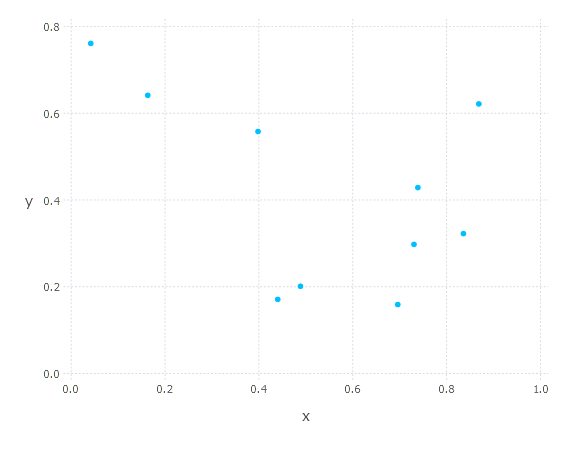
\includegraphics[height=4cm, keepaspectratio]{./figures/plot1.png}}
    \end{figure}
\end{center}
\end{frame}


\begin{frame}[containsverbatim]{\pq{Le dessin n'est pas la forme, il est la manière de voir la forme}{Edgar Degas}{goldenrod2}}
\par{Le paquet \cmdy{Gadfly} présente une syntaxe très proche de celle utilisée dans le package {\raisebox{-0.5ex}{\R}}: \cmdy{ggplot2}.}
\begin{lstlisting}[language=Julia, escapeinside={!*}{*!}]
p1 = plot(dta2, x = "statut", y = "x1", color = "statut")
\end{lstlisting}
\vspace{-2ex}
\begin{center}
    \begin{figure}
        \frame{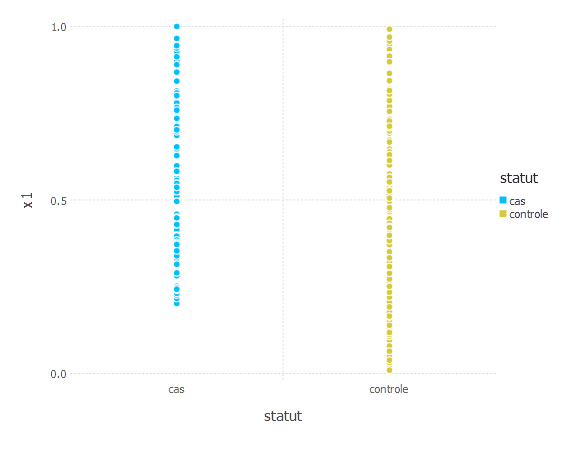
\includegraphics[height=4cm, keepaspectratio]{./figures/plot2.png}}
    \end{figure}
\end{center}
\end{frame}

\begin{frame}[containsverbatim]{\pq{Le dessin n'est pas la forme, il est la manière de voir la forme}{Edgar Degas}{goldenrod2}}
\begin{lstlisting}[language=Julia, escapeinside={!*}{*!}]
p2 = plot(
    dta2, x = "statut", y = "x1", color = "statut", Geom.boxplot,
    Scale.color_discrete_manual("firebrick2", "dodgerblue"),
    Guide.title("Le titre")
)
\end{lstlisting}
\vspace{-2ex}
\begin{center}
    \begin{figure}
        \frame{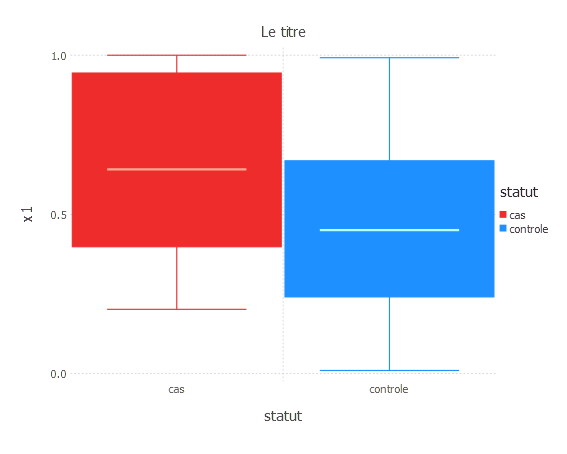
\includegraphics[height=4cm, keepaspectratio]{./figures/plot3.png}}
    \end{figure}
\end{center}
\end{frame}

\begin{frame}[containsverbatim]{\pq{Le dessin n'est pas la forme, il est la manière de voir la forme}{Edgar Degas}{goldenrod2}}
\begin{lstlisting}[language=Julia, escapeinside={!*}{*!}]
using PyPlot
surf(rand(30,40))
\end{lstlisting}
\vspace{-2ex}
\begin{center}
    \begin{figure}
        \frame{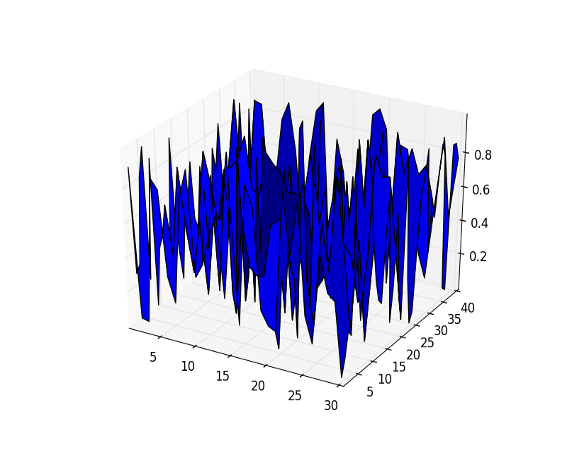
\includegraphics[height=4cm, keepaspectratio]{./figures/plot4.png}}
    \end{figure}
\end{center}
\end{frame}


\subsection{Les modules}
\begin{frame}[containsverbatim]{Les modules}
\par{{\Julia} propose un système de "\cmdy{module}" permettant d'encapsuler du code pour le (re)charger plus tard. Les paquets sont des modules.}
\begin{lstlisting}[language=Julia, escapeinside={!*}{*!}]
julia> module MonModule
           export x
           x = 1
           y = 2 # variable cachee
       end

julia> whos(MonModule)
MonModule                     Module
x                             Int64

julia> names(MonModule)
2-element Array{Symbol,1}:
 :MonModule
 :x

julia> x
!*\textcolor{firebrick2}{ERROR\hspace{-1.5ex}: x not defined}*!

julia> (MonModule.x, MonModule.y)
(1,2)
\end{lstlisting}
\end{frame}


\begin{frame}[containsverbatim]{Les modules}
\par{Pour (re)charger un module, il suffit d'utiliser la fonction \cmdb{using} de la même façon que pour un paquet.}
\begin{lstlisting}[language=Julia, escapeinside={!*}{*!}]
julia> using MonModule

julia> x
1

julia> y
!*\textcolor{firebrick2}{ERROR\hspace{-1.5ex}: y not defined}*!
\end{lstlisting}
\par{Il est également possible d'importer une fonction / variable d'un module, même si celle-ci n'a pas été exportée, via la fonction \cmdb{import}.}
\begin{lstlisting}[language=Julia, escapeinside={!*}{*!}]
julia> import MonModule.y

julia> y
2
\end{lstlisting}
\end{frame}


\subsection{Les macros}
\begin{frame}[containsverbatim]{Les macros}
\par{Les expressions (type \cmdg{Expr}), du code non évalué, sont définies avec\\\quad \cmdb{\hspace{-1.5ex}:( \cmd{...} )}}
\par{Elles peuvent être évaluées via la fonction \cmdb{eval()}.}
\begin{lstlisting}[language=Julia, escapeinside={!*}{*!}]
julia> :( println("Hello, world!") )
:(println("Hello, world!"))

julia> typeof(ans)
Expr

julia> eval(:( println("Hello, world!") ))
Hello, world!
\end{lstlisting}
\vspace{2ex}
\par{Les macros sont des fonctions commençant par le caractère \cmdb{@} et utilisant les expressions.}
\par{Elles sont définies avec les commandes de début \cmdb{macro} et de fin \cmdb{end}:}
\begin{lstlisting}[language=Julia, escapeinside={!*}{*!}]
julia> macro premieremacro(mot1, mot2)
    return :( println($mot1, $mot2) )
end
\end{lstlisting}
\end{frame}


\begin{frame}[containsverbatim]{Utiliser une macro}
\par{Les macros peuvent être utilisées de deux façons:}
\begin{lstlisting}[language=Julia, escapeinside={!*}{*!}]
julia> @premieremacro("Hello, ", "world!")
Hello, world!

julia> @premieremacro "Hello, " "world!"
Hello, world!
\end{lstlisting}
\vspace{2ex}
\par{\textcolor{firebrick2}{Attention, la seconde méthode peut être ambigüe lorsque des tuples sont utilisés.}}
\begin{lstlisting}[language=Julia, escapeinside={!*}{*!}]
@name expr1 expr2 # deux arguments

@name(expr1, expr2) # deux arguments

@name (expr1, expr2) # un argument, un tuple de deux elements
\end{lstlisting}
\end{frame}


\section{Appel de fonctions}
\subsection{Exécuter des commandes externes}
\begin{frame}[containsverbatim]{Exécuter des commandes externes}
\par{{\Julia} permet l'exécution de commandes externes:}
\begin{itemize}
\item avec \cmdb{run(`\cmd{...}`)}.
\begin{lstlisting}[language=Julia, escapeinside={!*}{*!}]
julia> run(`echo hello`)
hello
\end{lstlisting}
\item avec \cmdb{;} pour passer en mode console shell.
\begin{lstlisting}[language=Julia, escapeinside={!*}{*!}]
julia> ;
shell> echo hello
hello

julia>
\end{lstlisting}
\end{itemize}
\par{Dans les deux cas, le résultat n'est pas renvoyé dans {\Julia}. Pour récupérer le résultat d'une commande, il y a la fonction \cmdb{readall}.}
\begin{lstlisting}[language=Julia, escapeinside={!*}{*!}]
julia> res = readall(`echo hello`)
"hello\n"

julia> res
"hello\n"
\end{lstlisting}
\end{frame}


\subsection{Python}
\begin{frame}[containsverbatim]{Appel de fonctions Python}
\par{L'appel de fonctions Python s'effectue avec le paquet / module \cmdy{PyCall}.}
\begin{lstlisting}[language=Julia, escapeinside={!*}{*!}]
Pkg.add("PyCall")
using PyCall
\end{lstlisting}
\par{Les commandes \cmdb{pyeval} et \cmdb{pycall} permettent l'évaluation et l'exécution de commandes python, provenant d'une importation avec \cmdb{@pyimport}.}
\begin{lstlisting}[language=Julia, escapeinside={!*}{*!}]
julia> pyeval("1+1")
2

julia> @pyimport math # OR math = pyimport(:math)
PyObject <module 'math' from '/usr/lib64/python2.7/lib-dynload/math.so'>

julia> pycall(math["sin"], Float64, 1)
0.8414709848078965

julia> math.sin(math.pi / 4) - sin(pi / 4)
0.0
\end{lstlisting}
\vspace{-2ex}
\begin{lstlisting}[language=Julia, escapeinside={!*}{*!}]
@pyimport matplotlib.pyplot as plt
x = linspace(0,2*pi,1000); y = sin(3*x + 4*cos(2*x));
plt.plot(x, y, color="red", linewidth=2.0, linestyle="--");
plt.show()
\end{lstlisting}
\end{frame}


\subsection{C}
\begin{frame}[containsverbatim]{Appel de fonctions C}
\par{L'appel de fonctions C est possible nativement par {\Julia}.}
\par{Il passe par l'utilisation d'un \cmdy{tuple} contenant les informations sur la fonction et la librairie dans laquelle elle se trouve.}
\vspace{-2ex}
\begin{multicols}{2}
\begin{lstlisting}[language=Julia, escapeinside={!*}{*!}, xleftmargin=9mm, xrightmargin=2mm]
(:function, "library")
\end{lstlisting}
\columnbreak
\begin{lstlisting}[language=Julia, escapeinside={!*}{*!}, xleftmargin=2mm, xrightmargin=9mm]
("function", "library")
\end{lstlisting}
\end{multicols}
\vspace{-2ex}
\par{L'utilisation d'une fonction C passe par \cmdb{ccall}}
\begin{lstlisting}[language=Julia, escapeinside={!*}{*!}]
ccall(
    (:function, "library"), # tuple d'importation de la fonction
    ReturnType, # type du resultat renvoye par la fonction
    (InputType) # un tuple des types fournies en entree de la fonction
)
\end{lstlisting}
\vspace{-2ex}
\begin{lstlisting}[language=Julia, escapeinside={!*}{*!}]
julia> t = ccall( (:clock, "libc"), Int32, () )
34650000

julia> typeof(ans)
Int32
\end{lstlisting}
\end{frame}


\section{Aller plus loin avec Julia}
\begin{frame}[containsverbatim]{Aller plus loin avec Julia}
\begin{itemize}
\item Ce document est disponible sur \href{https://github.com/mcanouil/Presentation/tree/master/JULIA_TP}{GitHub}
\vspace{2ex}
\item Le site officiel: \href{http://julialang.org/}{http\hspace{-0.5ex}://julialang.org/}
\item La communauté: \href{http://julialang.org/community/}{http\hspace{-0.5ex}://julialang.org/community/}
\item La documentation complète: \href{http://docs.julialang.org/en/latest/}{http\hspace{-0.5ex}://docs.julialang.org/en/latest/}
\item Diverses sources d’informations: \href{http://julialang.org/learning/}{http\hspace{-0.5ex}://julialang.org/learning/}
\end{itemize}
\end{frame}

\section{Références}
\begin{frame}{Références}
    \bibliographystyle{apalike}
    \bibliography{./JULIA_biblio.bib}
    \nocite{*}
\end{frame}

\end{document}